\section{Additional Empirical Diagnostics}
\label{app:diagnostics}

% Appendix tables are numbered A1, A2, ...
\setcounter{table}{0}
\renewcommand{\thetable}{A\arabic{table}}
\setcounter{figure}{0}
\renewcommand{\thefigure}{A\arabic{figure}}

This appendix reports the detailed tables behind the synthetic-control, difference-in-differences, mechanism, and sectoral recovery results discussed in the main text. Tables are generated from stored result files by the original table script and the advisor-revision analysis scripts.

\subsection{Synthetic control}

\begin{table}[H]
\centering
\small
\caption{The full country sample and fitted national donor weights}
\label{tab:advisor_donors}
\begin{threeparttable}
\begin{tabular}{@{}lrrrr@{}}
\toprule
Country & Users & Pre mean (\%) & Pre SD (pp) & Weight (\%) \\
\midrule
Bangladesh & 10,241 & 17.25 & 3.60 & -- \\
Ghana & 1,373 & 17.03 & 2.24 & 32.49 \\
Indonesia & 10,965 & 15.71 & 2.09 & 0.00 \\
Jordan & 446 & 14.07 & 2.89 & 0.00 \\
Kenya & 3,553 & 18.58 & 3.70 & 19.93 \\
Malaysia & 1,396 & 14.87 & 1.85 & 0.00 \\
Morocco & 1,651 & 15.80 & 2.93 & 0.00 \\
Nepal & 2,373 & 16.56 & 1.62 & 0.00 \\
Nigeria & 6,961 & 16.52 & 2.07 & 0.00 \\
Pakistan & 7,276 & 14.48 & 1.96 & 47.58 \\
Philippines & 2,926 & 17.10 & 1.53 & 0.00 \\
Sri Lanka & 3,068 & 15.68 & 1.45 & 0.00 \\
Thailand & 2,317 & 15.49 & 1.47 & 0.00 \\
Tunisia & 1,012 & 14.21 & 2.54 & 0.00 \\
Vietnam & 3,600 & 16.76 & 1.82 & 0.00 \\
\bottomrule
\end{tabular}
\begin{tablenotes}[flushleft]
\footnotesize
\item The sample is unchanged. Pre-period: May 1--July 17. Every comparison country enters the fit; zero weight is an optimization result, not an exclusion. Bangladesh is the treated unit. Source: stored eligible-user and country-day panels; regenerated donor audit.
\end{tablenotes}
\end{threeparttable}
\end{table}

% Generated by analysis/tables/make_all_tables.py -- do not edit by hand.
\begin{table}[H]
\centering
\small
\caption{Primary synthetic-control donor weights}
\label{tab:weights}
\begin{threeparttable}
\begin{tabular*}{0.6\textwidth}{@{\extracolsep{\fill}}lr}
\toprule
Country & Weight \\
\midrule
Pakistan & 47.579\% \\
Ghana & 32.488\% \\
Kenya & 19.933\% \\
\bottomrule
\end{tabular*}
\begin{tablenotes}[flushleft]
\footnotesize\raggedright
\item \textit{Notes:} Weights are estimated on the pre-treatment (May 1--July 17, 2024) daily active-user rate. The remaining eleven donor countries receive zero weight.
\end{tablenotes}
\end{threeparttable}
\end{table}

% Generated by analysis/tables/make_all_tables.py -- do not edit by hand.
\begin{table}[H]
\centering
\footnotesize
\caption{Synthetic-control in-space placebo inference}
\label{tab:sc_placebos}
\begin{threeparttable}
\begin{tabular}{rlrrrr}
\toprule
Rank & Unit & ATT (pp) & Pre RMSPE & Post RMSPE & Ratio \\
\midrule
1 & \textbf{Bangladesh} & $-$13.256 & 3.260 & 13.666 & 4.192 \\
2 & Tunisia & $-$2.563 & 2.011 & 2.682 & 1.334 \\
3 & Nepal & 0.965 & 0.936 & 1.216 & 1.300 \\
4 & Jordan & $-$0.194 & 2.457 & 3.151 & 1.283 \\
5 & Indonesia & $-$1.393 & 1.151 & 1.462 & 1.270 \\
6 & Pakistan & 0.941 & 1.585 & 1.606 & 1.013 \\
7 & Kenya & 2.439 & 2.873 & 2.837 & 0.987 \\
8 & Nigeria & 0.527 & 0.948 & 0.823 & 0.869 \\
9 & Sri Lanka & $-$0.748 & 1.382 & 1.181 & 0.855 \\
10 & Thailand & $-$0.215 & 0.965 & 0.652 & 0.675 \\
11 & Ghana & 0.268 & 1.144 & 0.706 & 0.617 \\
12 & Vietnam & $-$0.097 & 0.867 & 0.458 & 0.528 \\
13 & Philippines & 0.091 & 0.955 & 0.416 & 0.435 \\
14 & Morocco & 0.050 & 1.794 & 0.625 & 0.348 \\
15 & Malaysia & 0.131 & 1.177 & 0.297 & 0.252 \\
\bottomrule
\end{tabular}
\begin{tablenotes}[flushleft]
\footnotesize\raggedright
\item \textit{Notes:} Each donor country is assigned the July 18--23 treatment in turn and its synthetic control is rebuilt from the remaining donors. Units are ordered by the post/pre RMSPE ratio. Bangladesh has both the largest ratio and the largest absolute ATT among the 15 units, so the exact rank $p$-value is $1/15=0.0667$ for both statistics. This is the minimum attainable value with 14 placebo countries; inference resolution is limited by the size of the donor pool.
\end{tablenotes}
\end{threeparttable}
\end{table}

% Generated by analysis/tables/make_all_tables.py -- do not edit by hand.
\begin{table}[H]
\centering
\small
\caption{Outcome-specific synthetic-control donor weights}
\label{tab:weights_specific}
\begin{threeparttable}
\begin{tabular}{llr}
\toprule
Outcome & Country & Weight \\
\midrule
Productive active rate & Pakistan & 36.1\% \\
 & Philippines & 25.2\% \\
 & Jordan & 21.3\% \\
 & Kenya & 16.5\% \\
 & Thailand & 0.8\% \\
\addlinespace Shipping active rate & Pakistan & 81.8\% \\
 & Ghana & 8.9\% \\
 & Morocco & 7.2\% \\
 & Jordan & 2.2\% \\
\addlinespace Collaboration active rate & Pakistan & 92.3\% \\
 & Morocco & 7.7\% \\
\addlinespace Collaboration events / 1,000 & Morocco & 84.7\% \\
 & Nigeria & 10.1\% \\
 & Ghana & 5.2\% \\
\addlinespace Shipping output / 1,000 & Pakistan & 72.5\% \\
 & Morocco & 8.4\% \\
 & Ghana & 8.2\% \\
 & Nigeria & 7.8\% \\
 & Philippines & 2.3\% \\
 & Jordan & 0.8\% \\
\bottomrule
\end{tabular}
\begin{tablenotes}[flushleft]
\footnotesize\raggedright
\item \textit{Notes:} Donors with zero weight are omitted. These weights are reported for transparency; the main secondary-outcome comparison holds the primary weights in \cref{tab:weights} fixed.
\end{tablenotes}
\end{threeparttable}
\end{table}

% Generated by analysis/tables/make_all_tables.py -- do not edit by hand.
\begin{table}[H]
\centering
\footnotesize
\caption{Synthetic difference-in-differences: sensitivity to the pre-treatment baseline}
\label{tab:sdid}
\begin{threeparttable}
\begin{tabular*}{0.85\textwidth}{@{\extracolsep{\fill}}lrr}
\toprule
Statistic & \multicolumn{2}{c}{Value} \\
\midrule
\multicolumn{3}{l}{\textit{A. Estimates, July 18--23, 2024 (pp)}} \\
Synthetic DiD (archived) & $-$17.9495 & -- \\
Canonical synthetic control (primary) & $-$13.256 & -- \\
\addlinespace \multicolumn{3}{l}{\textit{B. Decomposition by weighting scheme (pp)}} \\
Unit weights & SDID time weights & Uniform time weights \\
SDID unit weights & $-$17.95 & $-$13.86 \\
SC unit weights & $-$17.99 & $-$14.38 \\
Equal unit weights & $-$17.87 & $-$13.09 \\
\addlinespace \multicolumn{3}{l}{\textit{C. SDID time weights}} \\
Share of weight on July 1--17 & 72.2\% & \\
Weight on July 2 / July 10 & 27.1\% / 30.2\% & \\
Days with positive weight (of 78) & 14 & \\
Bangladesh baseline, SDID-weighted (\%) & 22.54 & \\
Bangladesh baseline, uniform pre-period mean (\%) & 17.25 & \\
\bottomrule
\end{tabular*}
\begin{tablenotes}[flushleft]
\footnotesize\raggedright
\item \textit{Notes:} Panel A: the archived SDID estimate \citep{arkhangelsky2021} and the primary synthetic control. The archived SDID standard error and $p$-value are not reported because their computation is undocumented. Panel B recomputes the point estimate from the archived SDID unit and time weights, replacing one set at a time; equal unit weights with uniform time weights reproduce the aggregate DiD. Panel C summarizes the archived time weights over May 1--July 17. Nothing is re-estimated. Sources: \texttt{results/synthetic\_control/main\_synthetic\_results.csv}, \texttt{sdid\_time\_weights.csv}, \texttt{donor\_weights.csv}; computed by \texttt{analysis/synthetic\_control/02\_sdid\_archived\_check.py}.
\end{tablenotes}
\end{threeparttable}
\end{table}


\begin{figure}[H]
\centering
\caption{Synthetic-control in-time placebos: ATT over six-day pseudo-treatment windows}
\label{fig:sc_intime}
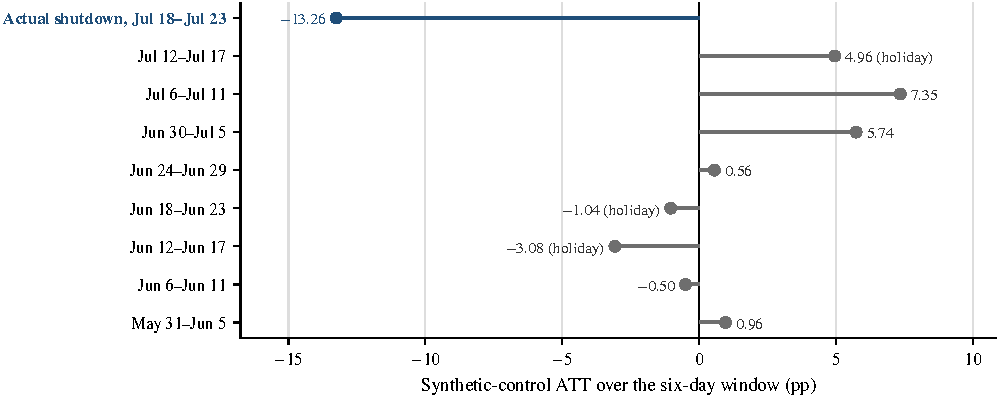
\includegraphics[width=\textwidth]{figA1_sc_intime_placebos.pdf}
\fignote{Each grey row is a six-day pre-treatment window chosen by the rule in \cref{sec:sc_diagnostics}; donor weights are re-estimated using only the days before each window, and the ATT is the mean gap between Bangladesh and its synthetic control over the window, as in the primary specification (blue row). ``Holiday'' marks windows containing a Bangladesh national holiday. All eight eligible windows are shown. Details in \cref{tab:sc_intime}. Source: \texttt{results/synthetic\_control/reproduced/sc\_intime\_placebos.csv}.}
\end{figure}

% Generated by analysis/tables/make_all_tables.py -- do not edit by hand.
\begin{table}[H]
\centering
\footnotesize
\caption{Synthetic-control in-time placebos}
\label{tab:sc_intime}
\begin{threeparttable}
\begin{tabular}{lrrrrrrl}
\toprule
Window (2024) & Fit days & ATT (pp) & Pre RMSPE & Ratio & Rank $|$ATT$|$ & Rank ratio & Holiday \\
\midrule
\textbf{Jul 18--Jul 23 (actual)} & 78 & $-$13.256 & 3.260 & 4.192 & 1 & 1 &  \\
Jul 12--Jul 17 & 72 & 4.958 & 3.032 & 1.787 & 4 & 5 & Ashura \\
Jul 6--Jul 11 & 66 & 7.349 & 2.279 & 3.376 & 2 & 3 &  \\
Jun 30--Jul 5 & 60 & 5.736 & 1.634 & 3.793 & 3 & 2 &  \\
Jun 24--Jun 29 & 54 & 0.560 & 1.685 & 0.654 & 8 & 9 &  \\
Jun 18--Jun 23 & 48 & $-$1.036 & 1.678 & 1.227 & 6 & 6 & Eid al-Adha \\
Jun 12--Jun 17 & 42 & $-$3.076 & 1.546 & 2.487 & 5 & 4 & Eid al-Adha \\
Jun 6--Jun 11 & 36 & $-$0.498 & 1.588 & 0.844 & 9 & 7 &  \\
May 31--Jun 5 & 30 & 0.964 & 1.683 & 0.720 & 7 & 8 &  \\
\bottomrule
\end{tabular}
\begin{tablenotes}[flushleft]
\footnotesize\raggedright
\item \textit{Notes:} Pre-specified rule: six-day pseudo-treatment windows, non-overlapping, moving backward from July 17, each with at least 28 days of fitting data from May 1. Donor weights are re-estimated for each window using only days before it; ATT and RMSPE definitions are those of the primary specification. Ranks are among the nine windows. The windows differ in fit length and are not exchangeable, so the ranks are descriptive and not a formal $p$-value. Source: \texttt{results/synthetic\_control/reproduced/sc\_intime\_placebos.csv}, computed by \texttt{analysis/synthetic\_control/03\_intime\_placebos.py}.
\end{tablenotes}
\end{threeparttable}
\end{table}


\subsection{International repository-domain diagnostics}
\label{app:sector_sc}

The following tables retain every country's coverage, all domain support decisions, and the fit and threshold diagnostics for the international extension. Missing estimates indicate insufficient support under the stated rule.

\begin{table}[H]
\centering
\small
\caption{International historical-text classification coverage}
\label{tab:sector_coverage}
\begin{threeparttable}
\begin{tabular}{@{}lrrrr@{}}
\toprule
Country & Eligible & README & Assigned & Assigned (\%) \\
\midrule
Bangladesh & 10,241 & 5,749 & 2,163 & 21.1 \\
Ghana & 1,373 & 892 & 318 & 23.2 \\
Indonesia & 10,965 & 6,810 & 2,678 & 24.4 \\
Jordan & 446 & 281 & 102 & 22.9 \\
Kenya & 3,553 & 2,264 & 870 & 24.5 \\
Malaysia & 1,396 & 916 & 343 & 24.6 \\
Morocco & 1,651 & 984 & 325 & 19.7 \\
Nepal & 2,373 & 1,272 & 444 & 18.7 \\
Nigeria & 6,961 & 4,442 & 1,552 & 22.3 \\
Pakistan & 7,276 & 4,209 & 1,512 & 20.8 \\
Philippines & 2,926 & 1,779 & 678 & 23.2 \\
Sri Lanka & 3,068 & 1,954 & 711 & 23.2 \\
Thailand & 2,317 & 1,526 & 581 & 25.1 \\
Tunisia & 1,012 & 577 & 230 & 22.7 \\
Vietnam & 3,600 & 2,182 & 898 & 24.9 \\
\bottomrule
\end{tabular}
\begin{tablenotes}[flushleft]
\footnotesize
\item Counts refer to users and their dominant pre-treatment repository. Assigned requires an available July 17 README and classifier score at least 0.80. Other eligible users remain unclassified; they are not removed from national estimates. Retrieval takes place in October 2026 and cannot recover every repository available in 2024.
\end{tablenotes}
\end{threeparttable}
\end{table}

\begin{table}[H]
\centering
\small
\caption{Pre-specified support screen for every domain}
\label{tab:sector_support}
\begin{threeparttable}
\begin{tabular}{@{}p{0.38\textwidth}rrr@{}}
\toprule
Domain & Bangladesh users & Eligible donors & Estimated \\
\midrule
Agriculture & 25 & 3 & No \\
Mining & 0 & 0 & No \\
Utilities & 8 & 0 & No \\
Construction & 1 & 0 & No \\
Manufacturing & 8 & 0 & No \\
Wholesale & 0 & 0 & No \\
Retail & 368 & 11 & Yes \\
Transport & 44 & 5 & Yes \\
Information & 518 & 14 & Yes \\
Finance & 90 & 9 & Yes \\
Real estate & 49 & 1 & No \\
Professional services & 151 & 11 & Yes \\
Administrative support & 36 & 1 & No \\
Education & 424 & 13 & Yes \\
Health & 155 & 5 & Yes \\
Arts and recreation & 72 & 7 & Yes \\
Accommodation and food & 192 & 4 & No \\
Other services & 18 & 1 & No \\
Public administration & 4 & 0 & No \\
Unclassified & 8078 & 14 & Yes \\
\bottomrule
\end{tabular}
\begin{tablenotes}[flushleft]
\footnotesize
\item At least 30 Bangladesh users and five donor countries with at least 30 users each are required. The rule uses sample support, not treatment-period effect size. Unreported estimates in the main table correspond to this screen, not a zero estimated effect.
\end{tablenotes}
\end{threeparttable}
\end{table}

\begin{table}[H]
\centering
\small
\caption{Sector-cohort fit and scale-adjusted placebo diagnostics}
\label{tab:sector_fit}
\begin{threeparttable}
\begin{tabular}{@{}p{0.27\textwidth}rrrr@{}}
\toprule
Domain & Pre RMSPE / mean & Holdout (pp) & Post/pre RMSPE & Ratio rank \\
\midrule
Retail & 0.15 & 3.57 & 5.43 & 0.083 \\
Transport & 0.51 & 5.16 & 1.96 & 0.167 \\
Information & 0.16 & 3.61 & 4.98 & 0.067 \\
Finance & 0.27 & 6.27 & 3.10 & 0.100 \\
Professional services & 0.24 & 5.24 & 4.18 & 0.083 \\
Education & 0.24 & 9.12 & 3.13 & 0.071 \\
Health & 0.32 & 6.20 & 2.40 & 0.167 \\
Arts and recreation & 0.31 & 6.65 & 2.32 & 0.125 \\
Unclassified & 0.20 & 7.50 & 3.89 & 0.067 \\
\bottomrule
\end{tabular}
\begin{tablenotes}[flushleft]
\footnotesize
\item The normalized fit divides pre-period RMSPE by mean pre-period activity. Holdout weights are fitted through June 30 and evaluated July 1--17, conditional on July 17 cohort definitions. Large errors limit counterfactual credibility. Ratio rank compares the shutdown/pre-period RMSPE ratio with sector-specific donor placebos.
\end{tablenotes}
\end{threeparttable}
\end{table}

\begin{table}[H]
\centering
\small
\caption{Sector-cohort ATT sensitivity to classification rules}
\label{tab:sector_sc_sensitivity}
\begin{threeparttable}
\begin{tabular}{@{}p{0.38\textwidth}rrrr@{}}
\toprule
Domain & 0.70 & 0.80 & 0.90 & Name fallback \\
\midrule
Accommodation and food & -14.56 & -- & -- & -15.71 \\
Arts and recreation & -11.61 & -12.33 & -- & -10.90 \\
Education & -16.30 & -15.04 & -15.83 & -14.15 \\
Finance & -10.97 & -12.28 & -12.10 & -12.59 \\
Health & -16.10 & -16.84 & -16.65 & -15.89 \\
Information & -13.07 & -12.74 & -12.50 & -12.70 \\
Professional services & -14.34 & -16.13 & -- & -16.13 \\
Retail & -16.47 & -15.69 & -15.16 & -14.31 \\
Transport & -10.95 & -11.31 & -- & -11.90 \\
Unclassified & -12.76 & -12.77 & -12.92 & -12.58 \\
\bottomrule
\end{tabular}
\begin{tablenotes}[flushleft]
\footnotesize
\item Effects in percentage points. The first three columns require a historical README. The final column admits classifications from names alone at score 0.80. Each rule changes the fixed cohort and may change donor support. A dash means insufficient support, not a zero effect; columns are therefore not estimates for an identical population.
\end{tablenotes}
\end{threeparttable}
\end{table}


\begin{figure}[H]
\centering
\caption{Observed and synthetic paths for all supported repository-domain cohorts}
\label{fig:advisor_sector_paths}
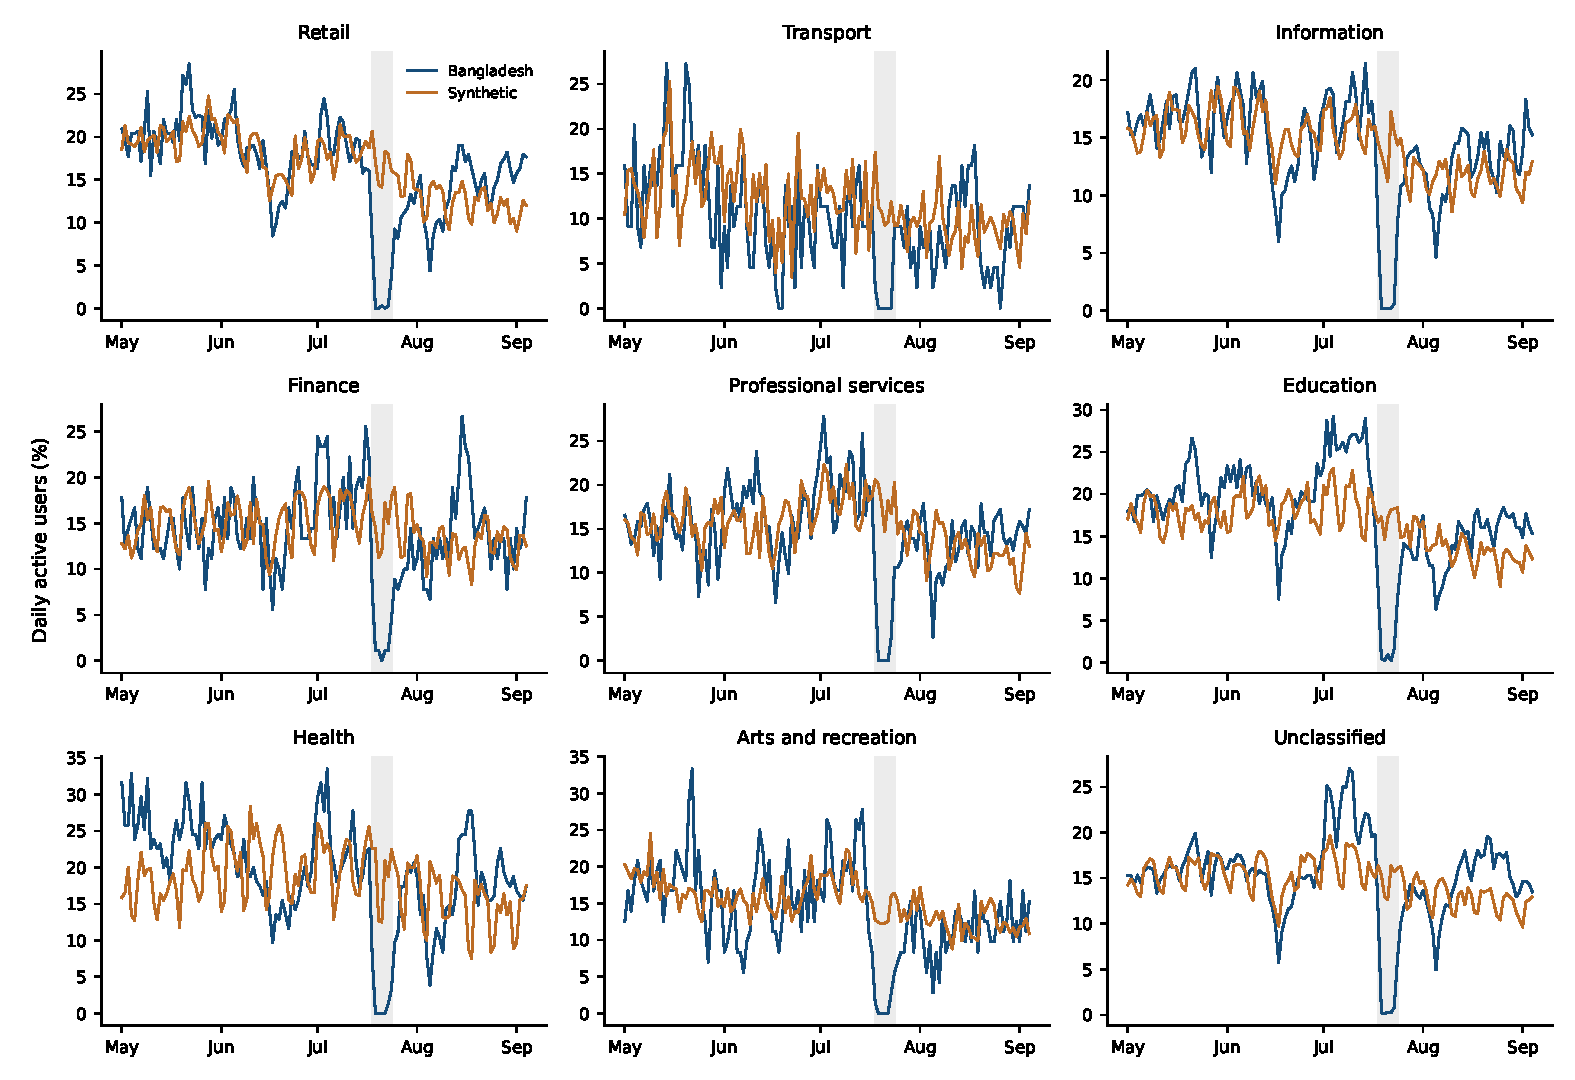
\includegraphics[width=\textwidth,height=0.76\textheight,keepaspectratio]{fig_advisor_sector_paths.pdf}
\fignote{Fixed pre-treatment user cohorts; historical README and score at least 0.80. Grey marks July 18--23, the primary estimand. Paths after July 23 are descriptive and use the same pre-fitted weights. Panel scales vary. Full domain-country weights, donor placebos and leave-one-out estimates are retained in the replication outputs.}
\end{figure}

\subsection{Difference-in-differences and event study}

% Generated by analysis/tables/make_all_tables.py -- do not edit by hand.
\begin{table}[H]
\centering
\footnotesize
\caption{Aggregate event study: all weekly estimates}
\label{tab:did_es_full}
\begin{threeparttable}
\begin{tabular}{lllrrrr}
\toprule
Week & Dates (2024) & Days & $\hat\theta_k$ (pp) & Placebo-based interval & Placebo range & Rank $p$ \\
\midrule
$-11$ & May 1--May 8 & 8 & $-$0.86 & [$-$4.37, 2.65] & [$-$1.68, 4.62] & 0.6000 \\
$-10$ & May 9--May 15 & 7 & $-$1.83 & [$-$4.50, 0.84] & [$-$2.23, 2.49] & 0.2667 \\
$-9$ & May 16--May 22 & 7 & 0.58 & [$-$1.21, 2.36] & [$-$1.06, 2.46] & 0.4667 \\
$-8$ & May 23--May 29 & 7 & $-$0.51 & [$-$2.47, 1.45] & [$-$2.36, 1.92] & 0.4667 \\
$-7$ & May 30--Jun 5 & 7 & $-$0.05 & [$-$2.08, 1.97] & [$-$1.72, 2.02] & 1.0000 \\
$-6$ & Jun 6--Jun 12 & 7 & $-$1.23 & [$-$3.28, 0.81] & [$-$0.99, 2.54] & 0.2000 \\
$-5$ & Jun 13--Jun 19 & 7 & $-$4.89 & [$-$9.31, $-$0.47] & [$-$3.64, 2.34] & 0.0667 \\
$-4$ & Jun 20--Jun 26 & 7 & $-$2.71 & [$-$5.13, $-$0.29] & [$-$3.06, 1.62] & 0.1333 \\
$-3$ & Jun 27--Jul 3 & 7 & 1.67 & [$-$0.46, 3.80] & [$-$1.31, 1.45] & 0.0667 \\
$-2$ & Jul 4--Jul 10 & 7 & 6.10 & [3.76, 8.43] & [$-$1.74, 1.62] & 0.0667 \\
$-1$ & Jul 11--Jul 17 & 7 & 3.86 & [2.15, 5.58] & [$-$1.63, 0.98] & 0.0667 \\
$0$ & Jul 18--Jul 23 & 6 & $-$13.09 & [$-$15.39, $-$10.79] & [$-$1.72, 1.60] & 0.0667 \\
$+1$ & Jul 24--Jul 30 & 7 & $-$2.66 & [$-$5.35, 0.02] & [$-$1.95, 2.23] & 0.0667 \\
$+2$ & Jul 31--Aug 6 & 7 & $-$2.76 & [$-$4.87, $-$0.65] & [$-$1.22, 2.56] & 0.0667 \\
$+3$ & Aug 7--Aug 13 & 7 & 0.52 & [$-$1.99, 3.02] & [$-$1.87, 2.73] & 0.9333 \\
$+4$ & Aug 14--Aug 20 & 7 & 4.31 & [1.99, 6.64] & [$-$1.82, 2.77] & 0.0667 \\
$+5$ & Aug 21--Aug 27 & 7 & 4.84 & [2.40, 7.28] & [$-$1.48, 2.71] & 0.0667 \\
$+6$ & Aug 28--Sep 3 & 7 & 2.53 & [0.01, 5.05] & [$-$2.32, 2.31] & 0.0667 \\
\bottomrule
\end{tabular}
\begin{tablenotes}[flushleft]
\footnotesize\raggedright
\item \textit{Notes:} $\hat\theta_k$ from \cref{eq:es_agg}, relative to the May 1--July 17 mean. Week $-11$ includes May 1; September 4 (a partial week) is omitted. \textit{Placebo range}: minimum and maximum of the 14 in-space placebo estimates. \textit{Placebo-based interval}: $\hat\theta_k\pm1.96$ times the placebo standard deviation; a donor-placebo reference interval, not a conventional confidence interval. Other definitions as in \cref{tab:did}. Source: \texttt{results/did/did\_eventstudy\_weekly.csv}.
\end{tablenotes}
\end{threeparttable}
\end{table}

% Generated by analysis/tables/make_all_tables.py -- do not edit by hand.
\begin{table}[H]
\centering
\footnotesize
\caption{International difference-in-differences by outcome}
\label{tab:did_secondary}
\begin{threeparttable}
\begin{tabular}{lrrrr}
\toprule
& \multicolumn{2}{c}{All days} & \multicolumn{2}{c}{Holidays excluded} \\
\cmidrule(lr){2-3}\cmidrule(lr){4-5}
Outcome & ATT & Relative & ATT & Relative \\
\midrule
Active-user rate (primary) & $-$13.088 & $-$86.6\% & $-$13.379 & $-$86.9\% \\
Productive active rate & $-$14.669 & $-$86.1\% & $-$14.975 & $-$86.3\% \\
Shipping active rate & $-$0.771 & $-$90.4\% & $-$0.806 & $-$90.8\% \\
Collaboration active rate & $-$0.302 & $-$84.9\% & $-$0.311 & $-$85.3\% \\
Collaboration events / 1,000 & $-$10.855 & $-$89.7\% & $-$11.532 & $-$90.2\% \\
Shipping output / 1,000 & $-$14.017 & $-$90.0\% & $-$14.631 & $-$90.4\% \\
\bottomrule
\end{tabular}
\begin{tablenotes}[flushleft]
\footnotesize\raggedright
\item \textit{Notes:} Aggregate DiD as in \cref{tab:did}, Panel A, for each outcome; rates in percentage points, counts per 1,000 eligible users. No placebo inference is stored for these specifications. Source: \texttt{results/final/table\_DiD\_all\_outcomes.csv}.
\end{tablenotes}
\end{threeparttable}
\end{table}



\subsection{Regression discontinuity in time}
\label{app:rdit_detail}
\label{sec:rdit_method}

A regression discontinuity in time provides a third temporal comparison. The archived preferred specification uses a cutoff at July 17, 2024, a bandwidth of $h=7$ days (July 10--24, fifteen daily observations), and a local linear fit on each side. With $\tilde{t} = t - \text{July 17}$ and $D_t = \mathbf{1}\{\tilde{t} \geq 0\}$, so that July 17 itself lies on the post-cutoff side, I estimate
\begin{equation}
  Y_{t} = \alpha + \tau D_{t} + \gamma_{1}\tilde{t} + \gamma_{2} D_{t}\tilde{t} + u_{t},
  \qquad |\tilde{t}| \leq h,
  \label{eq:rdit}
\end{equation}
where $\tau$ is the discontinuity and $Y_t$ is the daily share of users with at least one productive GitHub event in a balanced user-day panel of 10,329 Bangladesh-associated and 3,025 Philippines-associated accounts. This eligible sample differs slightly from the 10,241 Bangladesh accounts of the country-day panel used for the synthetic control. I estimate \cref{eq:rdit} for Bangladesh, for the Bangladesh-minus-Philippines gap as a controlled specification, and for the Philippines alone as a geographic placebo. Inference uses heteroskedasticity-and-autocorrelation-consistent (HAC) Newey--West standard errors with two lags, following the cautions in \citet{hausman2018} regarding serial correlation in time-series discontinuity designs. Because time itself is the running variable and other contemporaneous events can occur at the same date, the RDiT is interpreted as a robustness check rather than a standalone source of causal identification.

The July 17 cutoff reproduces the original preferred specification; it is not chosen because it yields a preferred estimate. No daily cutoff matches the event exactly: provider-level mobile outages began late on July 17 UTC, whereas the nationwide near-total cutoff occurred around 15:00 UTC on July 18 \citep{belson2024}. I therefore report a complete grid of July 17, 18, and 19 cutoffs crossed with 4-, 5-, 7-, 10-, and 14-day bandwidths in \cref{tab:rdit_grid}, together with the separate archived 16-specification grid in \cref{tab:rdit_arch_grid}. An hourly design would require a separate specification and is not pursued here.


\subsubsection{Results}
\label{sec:rdit_results}

\Cref{fig:rdit} shows the daily series used in the RDiT. In Bangladesh, the share of users with productive activity is 19.03 percent on July 17, falls to 10.74 percent on July 18, and lies between 0.48 and 1.23 percent from July 19 through July 23 before recovering gradually from July 24. The Philippines, used as a geographic placebo, shows no comparable break.

\begin{figure}[htbp]
\centering
\caption{Regression discontinuity in time: daily share of users with productive activity around the July 17 cutoff (visual companion to \cref{tab:rdit})}
\label{fig:rdit}
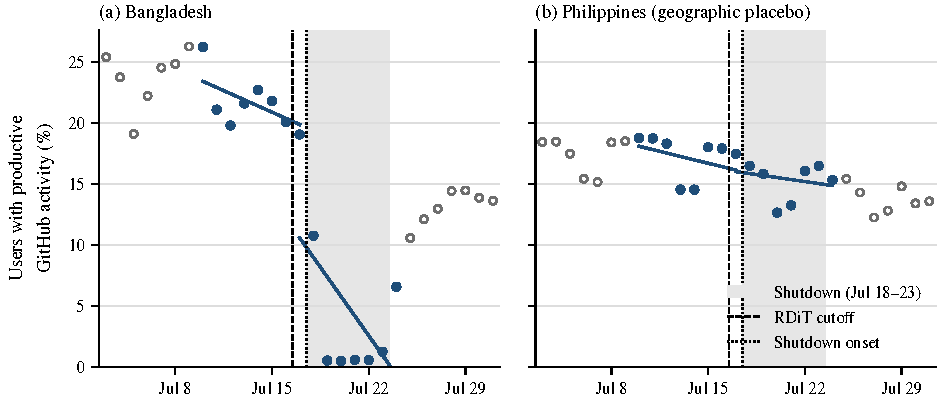
\includegraphics[width=\textwidth]{fig7_rdit_cutoff.pdf}
\fignote{Daily percentage of users with productive GitHub activity in the balanced user-day panels used for the RDiT (10,329 Bangladesh-associated and 3,025 Philippines-associated accounts). Filled markers are the fifteen days in the 7-day bandwidth of \cref{eq:rdit}. Lines are the fits of the archived preferred specification and correspond exactly to \cref{tab:rdit}. Dashed line: cutoff, with July 17 on the post-cutoff side; dotted line: shutdown boundary between July 17 and 18; shaded: July 18--23 shutdown. The RDiT is a temporal robustness check, not the primary design. Source: Author's calculations using GH Archive.}
\end{figure}

The RDiT produces a smaller point estimate but the same qualitative conclusion (\cref{tab:rdit}). The archived preferred local linear specification estimates a discontinuity of $-$9.28 percentage points in Bangladesh's active-user rate; a controlled Bangladesh-minus-Philippines version yields $-$9.16 percentage points. HAC $p$-values are approximately 0.065 in both cases, while the Philippines placebo is near zero. The smaller magnitude than in the synthetic control and DiD is consistent with the design visible in \cref{fig:rdit}: the cutoff day, July 17, precedes the shutdown but lies on the post-cutoff side, and the linear post-cutoff fit spans both the collapse and the beginning of the recovery on July 24.
Because \citet{hausman2018} urge caution in interpreting RDiT estimates, I emphasize the direction and timing of the break rather than treating the RDiT $p$-value as the decisive inferential statistic.

% Generated by analysis/tables/make_all_tables.py -- do not edit by hand.
\begin{table}[H]
\centering
\footnotesize
\caption{Regression discontinuity in time: preferred specification}
\label{tab:rdit}
\begin{threeparttable}
\begin{tabular}{l>{\raggedright\arraybackslash}p{3.3cm}rrcrr}
\toprule
Specification & Outcome & Effect (pp) & HAC SE & 95\% CI & $p$ & Days \\
\midrule
Main local linear & Bangladesh active rate & $-$9.284 & 5.034 & [$-$19.151, 0.584] & 0.065 & 15 \\
Controlled local linear & Bangladesh $-$ Philippines active rate & $-$9.160 & 4.980 & [$-$18.921, 0.601] & 0.066 & 15 \\
Geographic placebo & Philippines active rate & $-$0.124 & 1.492 & [$-$3.048, 2.801] & 0.934 & 15 \\
\bottomrule
\end{tabular}
\begin{tablenotes}[flushleft]
\footnotesize\raggedright
\item \textit{Notes:} Local linear RDiT at the July 17, 2024 cutoff, bandwidth 7 days, polynomial degree 1, no donut, HAC lags 2. Effects are reported in percentage points. RDiT is a temporal robustness check, not the primary causal design. Source: \texttt{results/rdit/main\_rdit\_summary.csv}.
\end{tablenotes}
\end{threeparttable}
\end{table}


The RDiT grid spans $-$4.45 to $-$19.52 percentage points for Bangladesh, illustrating substantial specification sensitivity (\cref{tab:rdit_grid}). The archived 16-row grid is also retained, but its input and cutoff provenance is unresolved. The RDiT sample includes 174 accounts absent from the main synthetic-control cohort, while 86 accounts in that cohort are absent from the RDiT sample; the difference is not simply 88 additional accounts. These facts limit a direct comparison of the two levels and estimates.


% Generated by analysis/tables/make_all_tables.py -- do not edit by hand.
\begin{table}[H]
\centering
\small
\caption{RDiT: complete cutoff and bandwidth grid}
\label{tab:rdit_grid}
\begin{threeparttable}
\begin{tabular*}{\textwidth}{@{\extracolsep{\fill}}llrrr}
\toprule
Cutoff & $h$ & Bangladesh & BD minus PH & Philippines \\
\midrule
07-17 & 4 & -4.45 (3.45) & -2.40 (3.43) & -2.05 (0.53) \\
07-17 & 5 & -7.30 (4.36) & -6.56 (4.87) & -0.74 (1.54) \\
07-17 & 7 & -9.28 (5.03) & -9.16 (4.98) & -0.12 (1.49) \\
07-17 & 10 & -13.70 (6.05) & -13.07 (5.80) & -0.62 (1.35) \\
07-17 & 14 & -16.80 (5.64) & -16.04 (5.35) & -0.76 (1.16) \\
07-18 & 4 & -11.09 (2.72) & -7.47 (2.14) & -3.62 (2.01) \\
07-18 & 5 & -12.98 (3.12) & -8.75 (1.94) & -4.24 (1.86) \\
07-18 & 7 & -17.49 (4.48) & -15.58 (4.29) & -1.91 (1.34) \\
07-18 & 10 & -18.06 (3.94) & -17.35 (4.18) & -0.71 (1.31) \\
07-18 & 14 & -19.52 (3.47) & -17.82 (3.50) & -1.70 (1.07) \\
07-19 & 4 & -9.00 (2.49) & -6.69 (2.12) & -2.31 (1.44) \\
07-19 & 5 & -11.54 (2.91) & -7.73 (1.99) & -3.81 (1.84) \\
07-19 & 7 & -16.59 (4.24) & -13.80 (4.06) & -2.79 (1.19) \\
07-19 & 10 & -16.76 (3.15) & -15.52 (3.59) & -1.23 (1.17) \\
07-19 & 14 & -17.60 (2.99) & -15.50 (3.16) & -2.10 (1.00) \\
\bottomrule
\end{tabular*}
\begin{tablenotes}[flushleft]
\footnotesize\raggedright
\item \textit{Notes:} All effects and HAC(2) standard errors in percentage points. Local linear fits with separate slopes, cutoff day on the right, inclusive symmetric bandwidth, $n/(n-4)$ variance correction. All 45 fits are reported; none replaces the archived July 17, $h=7$ result. Source: new round-2 diagnostic grid.
\end{tablenotes}
\end{threeparttable}
\end{table}

% Generated by analysis/tables/make_all_tables.py -- do not edit by hand.
\begin{table}[H]
\centering
\small
\caption{RDiT: preserved archived 16-specification grid}
\label{tab:rdit_arch_grid}
\begin{threeparttable}
\begin{tabular*}{\textwidth}{@{\extracolsep{\fill}}rlrrrr}
\toprule
Pre bandwidth & Polynomial & Donut & Effect (pp) & SE (pp) & $n$ \\
\midrule
7 & lin & False & -14.0 & 2.2 & 14 \\
7 & lin & True & -20.4 & 1.5 & 12 \\
7 & quad pre & False & -16.1 & 2.8 & 14 \\
7 & quad pre & True & -21.2 & 2.5 & 12 \\
10 & lin & False & -13.1 & 1.9 & 17 \\
10 & lin & True & -18.5 & 1.0 & 15 \\
10 & quad pre & False & -15.2 & 2.7 & 17 \\
10 & quad pre & True & -20.5 & 1.7 & 15 \\
14 & lin & False & -14.8 & 2.4 & 21 \\
14 & lin & True & -20.6 & 1.5 & 19 \\
14 & quad pre & False & -13.2 & 2.3 & 21 \\
14 & quad pre & True & -18.1 & 1.4 & 19 \\
21 & lin & False & -17.7 & 3.2 & 28 \\
21 & lin & True & -23.7 & 2.5 & 26 \\
21 & quad pre & False & -12.4 & 2.1 & 28 \\
21 & quad pre & True & -17.5 & 1.2 & 26 \\
\bottomrule
\end{tabular*}
\begin{tablenotes}[flushleft]
\footnotesize\raggedright
\item \textit{Notes:} Transcribed without re-estimation from data/processed/table3\_rdit\_sensitivity.csv. The historical cutoff, outcome, sample and variance procedure are not documented. The row labelled linear, 7 days, no donut is -14.0 pp, compared with -9.28 pp in the reproduced preferred specification; this is an unresolved provenance conflict, not evidence that one specification should replace the other.
\end{tablenotes}
\end{threeparttable}
\end{table}


\subsection{Mechanism}

\begin{table}[H]
\centering
\small
\caption{Repository-domain composition of residual-activity cohorts}
\label{tab:residual_domains}
\begin{threeparttable}
\begin{tabular}{@{}p{0.34\textwidth}rrrr@{}}
\toprule
Pre-treatment domain & \shortstack{All\\eligible} & \shortstack{Core\\publishers} & \shortstack{Onset\\authors} & \shortstack{Delayed\\authors} \\
\midrule
Accommodation and food & 192 & 0 & 4 & 3 \\
Administrative support & 36 & 0 & 0 & 0 \\
Agriculture & 25 & 0 & 1 & 1 \\
Arts and recreation & 72 & 0 & 4 & 2 \\
Construction & 1 & 0 & 0 & 0 \\
Education & 424 & 4 & 18 & 13 \\
Finance & 90 & 1 & 1 & 1 \\
Health & 155 & 0 & 5 & 3 \\
Information & 518 & 1 & 11 & 10 \\
Manufacturing & 8 & 0 & 0 & 0 \\
Other services & 18 & 0 & 0 & 0 \\
Professional services & 151 & 0 & 5 & 2 \\
Public administration & 4 & 0 & 0 & 0 \\
Real estate & 49 & 0 & 1 & 1 \\
Retail & 368 & 1 & 6 & 5 \\
Transport & 44 & 0 & 0 & 0 \\
Unclassified & 8,078 & 32 & 192 & 149 \\
Utilities & 8 & 1 & 2 & 1 \\
\bottomrule
\end{tabular}
\begin{tablenotes}[flushleft]
\footnotesize
\item Counts, not effects. Historical README classification at score 0.80; all unclassified accounts remain visible. Cohorts overlap and have the definitions in the mechanism section. Small cells and substantial unclassified coverage do not establish occupational specialization.
\end{tablenotes}
\end{threeparttable}
\end{table}


% Generated by analysis/tables/make_all_tables.py -- do not edit by hand.
\begin{table}[H]
\centering
\small
\caption{Mechanism placebo comparison}
\label{tab:mech_placebos}
\begin{threeparttable}
\begin{tabular}{lrrr}
\toprule
Metric & Real shutdown & Mean placebo & Maximum placebo \\
\midrule
Released in next 6 days & 25.38\% & 0.56\% & 0.77\% \\
Delay $>$24h & 29.71\% & 1.10\% & 1.31\% \\
Delay $>$48h & 25.38\% & 0.72\% & 0.90\% \\
Delay $>$72h & 22.75\% & 0.46\% & 0.56\% \\
Delay $>$120h & 13.88\% & 0.32\% & 0.46\% \\
\bottomrule
\end{tabular}
\begin{tablenotes}[flushleft]
\footnotesize\raggedright
\item \textit{Notes:} Placebo windows are six six-day authoring windows between July 1 and July 11, with six-day subsequent release windows that end before treatment. Windows overlap, so the comparison is descriptive rather than an exact independent randomization test.
\end{tablenotes}
\end{threeparttable}
\end{table}

% Generated by analysis/tables/make_all_tables.py -- do not edit by hand.
\begin{table}[H]
\centering
\footnotesize
\caption{Metadata coverage by push period}
\label{tab:metadata}
\begin{threeparttable}
\begin{tabular}{lrrrrr}
\toprule
Period & Target $N$ & Commit found & Author timestamp & Author login & Author = pusher \\
\midrule
Pre & 17,000 & 82.34\% & 82.34\% & 77.95\% & 71.49\% \\
Shutdown & 3,197 & 84.24\% & 84.24\% & 79.17\% & 69.69\% \\
Post & 65,868 & 81.81\% & 81.81\% & 77.81\% & 71.05\% \\
\bottomrule
\end{tabular}
\begin{tablenotes}[flushleft]
\footnotesize\raggedright
\item \textit{Notes:} Similar resolution rates across periods reduce concern that the mechanism result is generated by treatment-specific metadata missingness.
\end{tablenotes}
\end{threeparttable}
\end{table}

% Generated by analysis/tables/make_all_tables.py -- do not edit by hand.
\begin{table}[H]
\centering
\footnotesize
\caption{Push-listing completeness by period}
\label{tab:push_completeness}
\begin{threeparttable}
\begin{tabular}{lrrrrr}
\toprule
Period & Pushes & Mean push size & Complete pushes & Nominal commits & Commits in complete pushes \\
\midrule
Pre & 121,960 & 1.29 & 99.78\% & 157,834 & 90.27\% \\
Shutdown & 2,738 & 1.70 & 99.53\% & 4,667 & 73.11\% \\
Post & 58,110 & 1.69 & 99.66\% & 98,022 & 71.45\% \\
\bottomrule
\end{tabular}
\begin{tablenotes}[flushleft]
\footnotesize\raggedright
\item \textit{Notes:} A push is complete when its historical payload lists every commit. Large pushes account for a disproportionate share of commits and are more likely to be incomplete. Source: \texttt{results/mechanism/robust\_push\_size\_period.csv}.
\end{tablenotes}
\end{threeparttable}
\end{table}

% Generated by analysis/tables/make_all_tables.py -- do not edit by hand.
\begin{table}[H]
\centering
\footnotesize
\caption{Mechanism estimates by push size}
\label{tab:push_size}
\begin{threeparttable}
\begin{tabular}{lrrrrrr}
\toprule
Sample & $N$ & Backlog $N$ & Backlog share & $>$24h & $>$48h & $>$72h \\
\midrule
All complete pushes & 2,932 & 829 & 28.27\% & 29.71\% & 25.38\% & 22.75\% \\
Push size $\leq$ 10 & 2,503 & 526 & 21.01\% & 21.81\% & 18.98\% & 17.14\% \\
Push size $\leq$ 5 & 2,217 & 320 & 14.43\% & 15.07\% & 13.62\% & 12.45\% \\
Push size $\leq$ 2 & 1,947 & 151 & 7.76\% & 7.96\% & 7.29\% & 6.93\% \\
Single-commit pushes & 1,707 & 57 & 3.34\% & 3.28\% & 2.93\% & 2.75\% \\
\bottomrule
\end{tabular}
\begin{tablenotes}[flushleft]
\footnotesize\raggedright
\item \textit{Notes:} Strict \texttt{authoredDate} sample of commits authored July 18--23. The backlog share is not invariant to push size.
\end{tablenotes}
\end{threeparttable}
\end{table}

% Generated by analysis/tables/make_all_tables.py -- do not edit by hand.
\begin{table}[H]
\centering
\small
\caption{Concentration of the backlog across users and repositories}
\label{tab:concentration}
\begin{threeparttable}
\begin{tabular}{lr}
\toprule
Statistic & Value \\
\midrule
Shutdown-authored commits & 2,932 \\
Backlog commits & 829 (28.27\%) \\
Users / with backlog & 835 / 222 (26.59\%) \\
Repositories / with backlog & 977 / 246 (25.18\%) \\
Largest user's share of backlog & 2.77\% \\
Top 5 users' share of backlog & 12.06\% \\
Top 10 users' share of backlog & 21.47\% \\
\midrule \multicolumn{2}{l}{\textit{Backlog share after dropping top-$k$ backlog users}} \\
$k=1$ ($N=2,909$) & 27.71\% \\
$k=3$ ($N=2,868$) & 26.67\% \\
$k=5$ ($N=2,831$) & 25.75\% \\
$k=10$ ($N=2,739$) & 23.77\% \\
$k=20$ ($N=2,577$) & 20.37\% \\
\bottomrule
\end{tabular}
\begin{tablenotes}[flushleft]
\footnotesize\raggedright
\item \textit{Notes:} Strict \texttt{authoredDate} sample. Users are ranked by their number of backlog commits.
\end{tablenotes}
\end{threeparttable}
\end{table}


\subsection{Within-Bangladesh sectoral recovery}
\label{sec:sector_method}

The designs above estimate the effect of the shutdown during July 18--23. To describe how activity evolved after restoration, I use the fixed sample of 20,000 accounts described in \cref{sec:sector_data}. For user $i$, sector $s$, and day $t$, let $A_{ist}=1$ if the user records at least one PushEvent on day $t$ in a repository classified to sector $s$; activity in several repositories of the same sector on the same day counts once. Days are grouped into event periods $k$: the final eight complete pre-shutdown weeks, $k=-8,\dots,-1$ (May 23--July 17, 2024); the shutdown, $k=0$ (July 18--23); and consecutive seven-day bins after it, starting with $k=+1$ (July 24--30). Let $\bar{A}_{isk}$ be user $i$'s share of active days in period $k$, and $\bar{A}^{\mathrm{pre}}_{is}$ the corresponding share over the 56 baseline days. I report
\begin{equation}
  \beta_{sk} = \frac{100}{N}\sum_{i=1}^{N}\bigl(\bar{A}_{isk} - \bar{A}^{\mathrm{pre}}_{is}\bigr),
  \qquad
  R_{sk} = 100 \times \frac{\sum_{i} \bar{A}_{isk}}{\sum_{i} \bar{A}^{\mathrm{pre}}_{is}},
  \label{eq:sector}
\end{equation}
where $N=20{,}000$ and users without activity in sector $s$ contribute zeros. The coefficient $\beta_{sk}$ is the change in the daily probability of sector-$s$ push activity relative to the baseline, in percentage points; the recovery index $R_{sk}$ normalizes the baseline to 100. Standard errors for $\beta_{sk}$ are 100 times the standard deviation of the user-level differences divided by $\sqrt{N}$, and 95 percent intervals use the normal approximation. As a summary of recovery timing, I report the first post-shutdown week that begins two consecutive weeks with $R_{sk}\geq 80$.

Because the activity measure counts pushes to any classified repository, including repositories first observed after the shutdown, it captures recovery through new projects and through switching across repositories. As a complementary specification, I also follow only the repositories pushed to during the baseline weeks, whose activity cannot be replaced by new projects.

This analysis compares each sector with its own pre-shutdown baseline and has no untreated comparison group. It therefore describes the heterogeneity and timing of recovery within Bangladesh; it does not estimate sector-specific causal effects. Post-shutdown deviations from the baseline may also reflect trends, seasonality, or other Bangladesh-specific developments. The confidence intervals capture sampling variation across users but not common shocks that affect all users in a given week. The pre-shutdown coefficients ($k<0$) indicate how much weekly activity fluctuates around the baseline in the absence of a shutdown and serve as a benchmark for interpreting post-shutdown deviations.

\subsection{Sectoral recovery after restoration}
\label{sec:sector_results}

The synthetic-control estimates describe the collapse during the shutdown window. They do not show how activity evolved once connectivity returned, or whether recovery was common across the kinds of projects on which Bangladeshi developers work. This subsection addresses both questions using the fixed sample of 20,000 Bangladesh-associated accounts and the repository-sector classification of \cref{sec:sector_data}, estimated as described in \cref{sec:sector_method}. The analysis compares each sector with its own pre-shutdown baseline. It documents heterogeneity in recovery dynamics within Bangladesh; it does not estimate sector-specific causal effects relative to an untreated international control, and the synthetic-control estimate in \cref{sec:main_results} remains the paper's headline result. Throughout, a sector refers to the economic sector associated with the repositories in which observable GitHub activity occurs, not to developers' employers or industries of employment.

% Generated by analysis/tables/make_all_tables.py -- do not edit by hand.
\begin{table}[htbp]
\centering
\footnotesize
\caption{Recovery of observable GitHub push activity by repository sector}
\label{tab:sector_recovery}
\begin{threeparttable}
\begin{tabular}{lrrrrrrrrr}
\toprule
& & Pre & Pre rate & \multicolumn{5}{c}{Recovery index (pre-period mean = 100)} & First wk \\
\cmidrule(lr){5-9}
Sector & NAICS & users & (\%) & Shutdown & +1 & +2 & +4 & +8 & $\geq$80, 2 wks \\
\midrule
Finance & 52 & 382 & 0.078 & 30.9 & 92.2 & 67.6 & 89.5 & 91.3 & 3 \\
Information & 51 & 1,528 & 0.442 & 11.7 & 75.9 & 72.2 & 106.0 & 94.5 & 3 \\
Education & 61 & 1,234 & 0.385 & 11.7 & 59.1 & 53.4 & 75.4 & 81.9 & 6 \\
Health & 62 & 514 & 0.132 & 6.3 & 40.7 & 51.5 & 77.5 & 89.4 & 6 \\
Retail & 44--45 & 1,012 & 0.295 & 6.2 & 52.0 & 52.3 & 153.7 & 79.6 & 9 \\
Real Estate & 53 & 213 & 0.063 & 4.0 & 33.0 & 25.1 & 44.4 & 85.5 & 5 \\
Accommodation/Food & 72 & 480 & 0.144 & 3.5 & 44.3 & 42.8 & 54.2 & 62.6 & -- \\
\bottomrule
\end{tabular}
\begin{tablenotes}[flushleft]
\footnotesize\raggedright
\item \textit{Notes:} Fixed sample of 20,000 Bangladesh-associated accounts. Repository sectors from the historical-README classifier with confidence $\geq$ 0.80. The outcome is the share of sampled users with at least one PushEvent to a repository of the sector on a given day. \textit{Pre users}: sampled users with such activity in the baseline period. \textit{Pre rate}: mean daily outcome over the baseline period (May 23--July 17, 2024, the final eight complete pre-shutdown weeks), in percent of all 20,000 users. Shutdown: July 18--23; week +1: July 24--30; subsequent 7-day bins. \textit{First wk $\geq$80, 2 wks}: first post-shutdown week that begins two consecutive weeks with an index of at least 80 (observed through week +17, November 13--19); it does not imply that the index stays above 80 thereafter. -- indicates no such week. Within-Bangladesh comparison with the sector's own pre-period; not a causal effect relative to an untreated control. Sources: \texttt{results/sector\_recovery/sectorwide/sectorwide\_recovery\_summary.csv}, verified against \texttt{results/sector\_recovery/final/table\_sector\_recovery\_main.csv}.
\end{tablenotes}
\end{threeparttable}
\end{table}


All seven sectors show a sharp fall in observable push activity during July 18--23 (\cref{tab:sector_recovery,fig:sector_index}). The shutdown-period recovery index ranges from 3.5 in Accommodation/Food to 11.7 in Information and Education and 30.9 in Finance. In every sector, the 95 percent confidence interval for the change relative to the baseline excludes zero (Appendix \cref{fig:sector_es}).

Restoration of connectivity did not imply an immediate or uniform recovery. In the first week after the shutdown (July 24--30), the recovery index ranges from 33.0 in Real Estate to 92.2 in Finance. Mobile connectivity returned only during this week, later than fixed broadband \citep{belson2024}, so part of the week $+1$ shortfall may reflect incomplete restoration. Recovery was also not monotonic: in Finance, Information, Education, Real Estate, and Accommodation/Food, the index is lower in week $+2$ (July 31--August 6) than in week $+1$. This week includes the renewed mobile shutdown on August 4 and the nationwide disruption on August 5 \citep{belson2024q3}, alongside unrest and initially declared holidays. These overlapping events prevent a separate attribution of the second-week decline. The stored holiday labels extend through August 7, although offices were ordered to reopen on August 6 \citep{bss2024reopen}; I keep the stored labels and document the discrepancy in the replication materials.

\begin{figure}[htbp]
\centering
\caption{Recovery of observable GitHub push activity by repository sector}
\label{fig:sector_index}
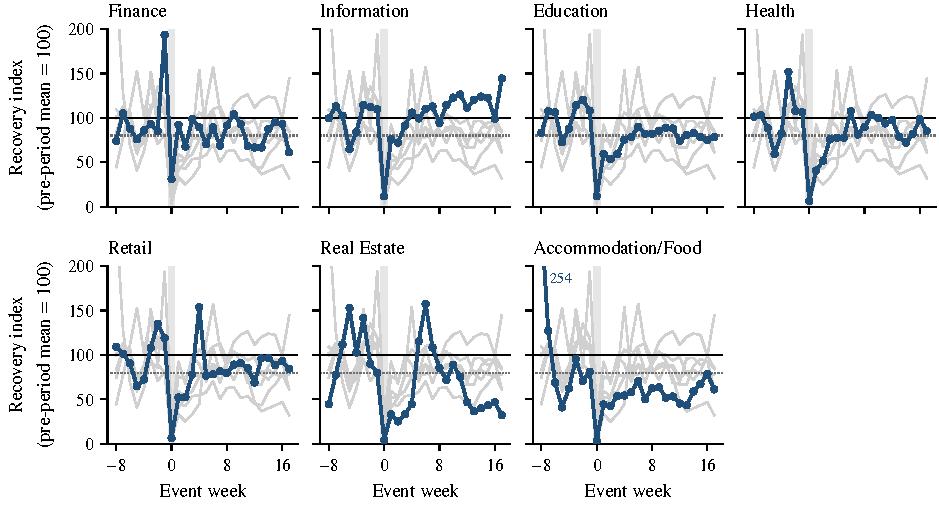
\includegraphics[width=\textwidth]{fig5_sector_recovery_index.pdf}
\fignote{Each panel highlights one sector's recovery index $R_{sk}$ (\cref{eq:sector}), 100 times its mean daily probability of push activity in event week $k$ relative to May 23--July 17, 2024; other sectors in grey. Shaded: July 18--23 shutdown; week $+1$ is July 24--30, and the window ends at week $+17$ (November 13--19). Lines mark 100 and 80; the one value above 200 is labeled. Fixed sample of 20,000 Bangladesh-associated accounts; sectors from a README classifier with confidence $\geq 0.80$ \citep{quispe2026naics} describe the repositories in which activity occurs, not developers' employers. Within-Bangladesh descriptive comparison, not a causal effect. Source: Author's calculations using GH Archive.}
\end{figure}

Finance and Information recovered fastest. Finance returned to an index of 92.2 in week $+1$, and both sectors begin a run of two consecutive weeks at or above 80 in week $+3$. Information exceeds its baseline by week $+4$ (106.0). In week $+8$, Finance is 91.3 and Information is 94.5. The Finance series is nonetheless noisy: its baseline includes a spike in week $-1$ (index 193.6), and its post-shutdown index falls back below 80 in several later weeks.

Education and Health recovered more gradually. Their week $+1$ indices are 59.1 and 40.7, they reach 75.4 and 77.5 by week $+4$, and both begin a run of two consecutive weeks at or above 80 only in week $+6$. By week $+8$, they stand at 81.9 and 89.4.

Accommodation/Food remained persistently depressed. Its index is 44.3 in week $+1$, 54.2 in week $+4$, and 62.6 in week $+8$, and it never records two consecutive weeks at or above 80 through the end of the observation window (week $+17$, November 13--19). This result should be read alongside the sector's unstable baseline: the index is 254.1 and 127.3 in the first two baseline weeks and between 40.8 and 95.5 in the remaining six. Part of the post-shutdown gap may therefore reflect a decline that began before the shutdown rather than a failure to recover.

Real Estate recovered slowly at first and later approached its baseline. Its index remains between 25.1 and 44.4 through week $+4$, rises above 100 in weeks $+5$, $+6$ and $+7$ (115.1, 157.3 and 108.3), and is 85.5 in week $+8$. This later recovery is not durable within the observed window: from week $+12$ onward, the index lies between 31.9 and 46.7 (\cref{fig:sector_index}). Real Estate is also the smallest of the seven sectors, with 213 sampled users active in the baseline period, so its weekly estimates are imprecise.

Retail shows a pronounced temporary rebound. Its index is about 52 in weeks $+1$ and $+2$, rises to 153.7 in week $+4$ (August 14--20), and falls back to 76.5 in week $+5$. Its first run of two consecutive weeks at or above 80 begins only in week $+9$. The week $+4$ value is therefore a transient overshoot, possibly reflecting a burst of catch-up activity, rather than evidence of completed recovery; the data do not identify what generated it. The timing of Retail's first two-week run is also sensitive to the classifier threshold (\cref{sec:sector_robustness}).

Index values above 100 later in the window should not be read as gains caused by the shutdown. Information, for example, has an index between 111.5 and 126.3 in weeks $+10$ to $+15$ and 144.3 in week $+17$. Without an untreated comparison group, such movements cannot be separated from trend growth, seasonality, or changes in the sampled users' activity.

The main specification counts pushes to any classified repository, including repositories first observed after the shutdown. A complementary specification follows only repositories pushed to during the eight baseline weeks (\cref{tab:sector_fixed_repo}). Activity in these pre-existing repositories recovers far less: in week $+8$, their indices range from 10.1 (Accommodation/Food) to 31.4 (Education), compared with 62.6 to 94.5 in the sector-wide specification. Because repositories selected on recent activity would become less active over time even without a shutdown, this gap does not measure a shutdown effect. It is nevertheless consistent with recovery occurring partly through new repositories and switching across projects rather than solely through a return to pre-existing ones.

Taken together, the sectoral evidence indicates that the collapse in observable activity documented in \cref{sec:main_results} was followed by a recovery that was gradual and uneven across the economic sectors associated with developers' repositories. These are before--after comparisons within Bangladesh. They share the identification limitations discussed in \cref{sec:unrest} and, in addition, cannot separate post-shutdown recovery from other Bangladesh-specific developments between August and November 2024.

\subsubsection{Additional sector-recovery diagnostics}

\begin{figure}[H]
\centering
\caption{Sectoral event study: change in daily push-activity probability relative to the pre-shutdown baseline}
\label{fig:sector_es}
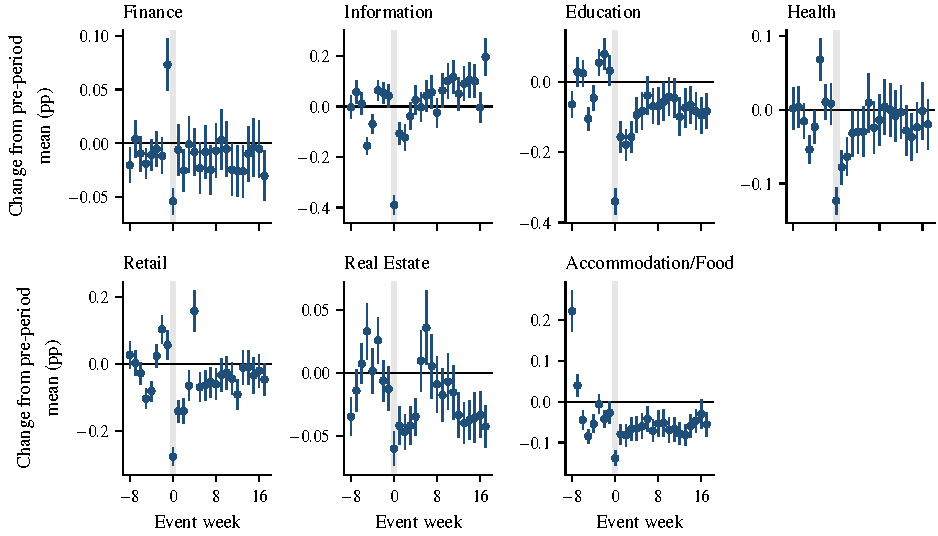
\includegraphics[width=\textwidth]{fig6_sector_eventstudy.pdf}
\fignote{Points are $\beta_{sk}$ from \cref{eq:sector}: the mean change, across the fixed sample of 20,000 Bangladesh-associated accounts, in the daily probability of a PushEvent in a sector-$s$ repository during event week $k$, relative to each user's mean over May 23--July 17, 2024, in percentage points. Vertical lines are 95 percent confidence intervals from the cross-user standard deviation of these differences; they capture sampling variation across users but not common weekly shocks. Shaded: July 18--23 shutdown; the window ends at week $+17$ (November 13--19). Vertical scales differ across panels. Within-Bangladesh descriptive comparison, not a causal effect relative to an untreated control. Source: Author's calculations using GH Archive.}
\end{figure}

% Generated by analysis/tables/make_all_tables.py -- do not edit by hand.
\begin{table}[H]
\centering
\footnotesize
\caption{Sectoral recovery indices by classifier-confidence threshold}
\label{tab:sector_threshold}
\begin{threeparttable}
\begin{tabular}{llrrrrr}
\toprule
Sector & Threshold & Pre users & Week +1 & Week +4 & Week +8 & First wk $\geq$80, 2 wks \\
\midrule
Finance & 0.70 & 437 & 91.6 & 92.4 & 89.2 & 3 \\
 & 0.80 & 382 & 92.2 & 89.5 & 91.3 & 3 \\
 & 0.90 & 275 & 101.7 & 82.5 & 101.7 & 3 \\
Information & 0.70 & 2,123 & 73.0 & 116.6 & 101.3 & 3 \\
 & 0.80 & 1,528 & 75.9 & 106.0 & 94.5 & 3 \\
 & 0.90 & 968 & 79.5 & 97.6 & 91.5 & 3 \\
Education & 0.70 & 1,345 & 61.6 & 75.4 & 79.4 & 5 \\
 & 0.80 & 1,234 & 59.1 & 75.4 & 81.9 & 6 \\
 & 0.90 & 1,029 & 57.8 & 73.3 & 77.0 & 6 \\
Health & 0.70 & 542 & 40.8 & 76.4 & 88.3 & 6 \\
 & 0.80 & 514 & 40.7 & 77.5 & 89.4 & 6 \\
 & 0.90 & 455 & 41.1 & 75.5 & 87.6 & 8 \\
Retail & 0.70 & 1,090 & 52.2 & 159.1 & 82.5 & 4 \\
 & 0.80 & 1,012 & 52.0 & 153.7 & 79.6 & 9 \\
 & 0.90 & 829 & 50.1 & 157.4 & 80.9 & 7 \\
Real Estate & 0.70 & 228 & 33.1 & 45.5 & 90.0 & 5 \\
 & 0.80 & 213 & 33.0 & 44.4 & 85.5 & 5 \\
 & 0.90 & 153 & 44.9 & 44.9 & 75.5 & 5 \\
Accommodation/Food & 0.70 & 514 & 46.0 & 59.3 & 64.9 & -- \\
 & 0.80 & 480 & 44.3 & 54.2 & 62.6 & -- \\
 & 0.90 & 394 & 39.2 & 45.1 & 60.3 & -- \\
\midrule \multicolumn{7}{l}{\textit{Excluded from the main figures and table}} \\
Professional/Scientific & 0.70 & 1,241 & 57.9 & 66.9 & 91.2 & 7 \\
 & 0.80 & 577 & 64.9 & 64.9 & 91.0 & 7 \\
 & 0.90 & 125 & 94.4 & 65.6 & 78.7 & 1 \\
Admin. Support & 0.70 & 268 & 30.8 & 83.0 & 77.0 & 9 \\
 & 0.80 & 196 & 32.2 & 72.9 & 84.7 & 10 \\
 & 0.90 & 48 & 5.2 & 61.9 & 56.8 & -- \\
\bottomrule
\end{tabular}
\begin{tablenotes}[flushleft]
\footnotesize\raggedright
\item \textit{Notes:} Each row repeats the main specification (\cref{tab:sector_recovery}) keeping only repositories whose classifier confidence is at least the stated threshold; 0.80 is the main specification. Professional/Scientific and Administrative Support are excluded from the main results because their support falls sharply at the 0.90 threshold. Source: \texttt{results/sector\_recovery/final/sector\_threshold\_robustness\_full.csv}.
\end{tablenotes}
\end{threeparttable}
\end{table}

% Generated by analysis/tables/make_all_tables.py -- do not edit by hand.
\begin{table}[H]
\centering
\footnotesize
\caption{Recovery of pre-existing repositories versus sector-wide user activity}
\label{tab:sector_fixed_repo}
\begin{threeparttable}
\begin{tabular}{lrrrrrrr}
\toprule
& & \multicolumn{3}{c}{Fixed pre-period repositories} & \multicolumn{3}{c}{Sector-wide (main)} \\
\cmidrule(lr){3-5}\cmidrule(lr){6-8}
Sector & Repos & +1 & +4 & +8 & +1 & +4 & +8 \\
\midrule
Finance & 417 & 60.0 & 28.3 & 23.0 & 92.2 & 89.5 & 91.3 \\
Information & 2,040 & 46.8 & 37.4 & 27.3 & 75.9 & 106.0 & 94.5 \\
Education & 1,523 & 40.3 & 38.2 & 31.4 & 59.1 & 75.4 & 81.9 \\
Health & 651 & 25.1 & 28.6 & 23.1 & 40.7 & 77.5 & 89.4 \\
Retail & 1,322 & 28.7 & 30.9 & 19.8 & 52.0 & 153.7 & 79.6 \\
Real Estate & 254 & 16.1 & 25.7 & 30.0 & 33.0 & 44.4 & 85.5 \\
Accommodation/Food & 581 & 29.4 & 16.1 & 10.1 & 44.3 & 54.2 & 62.6 \\
\bottomrule
\end{tabular}
\begin{tablenotes}[flushleft]
\footnotesize\raggedright
\item \textit{Notes:} Recovery indices (pre-period mean = 100). \textit{Fixed pre-period repositories}: classified repositories (confidence $\geq$ 0.80) with at least one PushEvent by a sampled user during the final eight pre-shutdown weeks; the outcome is each repository's daily PushEvent active-day rate, and new repositories never enter. \textit{Sector-wide}: main specification of \cref{tab:sector_recovery}, which includes activity on repositories first observed after the shutdown. Because a cohort selected on recent activity would decline over time even without a shutdown, the fixed-repository indices are not a counterfactual for the sector-wide indices. Sources: \texttt{results/sector\_recovery/pre8/sector\_recovery\_summary\_pre8.csv} and \texttt{results/sector\_recovery/sectorwide/sectorwide\_recovery\_summary.csv}.
\end{tablenotes}
\end{threeparttable}
\end{table}


\clearpage
\subsection{Connectivity chronology and threats to the comparison}
\label{app:connectivity_audit}

The connectivity record is useful both for defining exposure and for assessing the comparison series. Network traffic is not itself a measure of GitHub production, and a provider-level disruption need not affect every account in a country. The following review records documented events within the May 1--September 4 observation period. Absence from these non-exhaustive reports is not evidence of uninterrupted connectivity.

\begin{table}[htbp]
\centering\small
\caption{Documented connectivity events relevant to the analysis}
\label{tab:evidence_connectivity}
\begin{threeparttable}
\begin{tabular}{@{}p{.14\textwidth}p{.16\textwidth}p{.36\textwidth}p{.25\textwidth}@{}}
\toprule
Country & Date (2024) & Documented event & Implication \\
\midrule
Bangladesh & July 18 & Near-zero national traffic around 15:00 UTC \citep{belson2024} & Daily July 18 includes pre-cut hours. \\
Bangladesh & July 23 & Broadband recovery at 13:00 UTC in the August report, 12:00 UTC in Q3 \citep{belson2024,belson2024q3} & Both endpoints retained in author-cohort counts. \\
Bangladesh & July 28 & Major mobile networks recover around 09:00 UTC \citep{belson2024} & Restoration differs across access networks. \\
Bangladesh & August 4--5 & Renewed mobile outage, followed by national interruption on August 5 \citep{belson2024q3} & Later dip has additional network exposure. \\
Kenya & May 2; May 12 & Power-related disruption; submarine-cable failures \citep{cloudflare2024} & Pre-period donor contamination. \\
Kenya & June 25 & Large traffic disruption during protests; cause disputed \citep{cloudflare2024} & Connectivity and unrest are not separated. \\
Kenya & August 30--31 & Power-outage disruption \citep{belson2024q3} & Later synthetic path may be depressed. \\
Pakistan & July 31 & About two hours of disruption, with roughly 45\% national traffic decline \citep{belson2024} & Outside primary window; affects recovery comparison. \\
Nepal & May 2; June 3 & Provider outages associated with upstream payments and routing \citep{cloudflare2024} & Exposure differs by provider. \\
Malaysia & May 21 & Celcom disruption; a separate apparent dip was a Cloudflare processing issue \citep{cloudflare2024} & Telemetry artefacts must not be coded as outages. \\
\bottomrule\end{tabular}
\begin{tablenotes}[flushleft]\footnotesize
\item Times are UTC. This source audit does not change the donor pool or refit weights. Pakistan's regional July restrictions are discussed in the main donor diagnostics. The August 6 reopening reported by BSS conflicts with August 6--7 holiday labels in the input panel; the original labels and separate sensitivity remain documented. Kenya and Pakistan have positive national weights, so their post-window disruptions are especially relevant to apparent catch-up. No causal GitHub effect is assigned to a listed event solely because it appears in the chronology.
\end{tablenotes}\end{threeparttable}
\end{table}

\clearpage
\subsection{Detailed residual-publication audit}
\label{app:residual_audit}

\begin{table}[htbp]
\centering\small
\caption{Pre-period activity and the automation component of residual publication}
\label{tab:evidence_features}
\begin{threeparttable}
\begin{tabular}{@{}p{0.38\textwidth}rrrr@{}}
\toprule
Group & Users & Active days (\%) & Pushes & Fri--Sat (\%) \\
\midrule
All eligible & 10,241 & 17.25 & 21.0 & 25.96 \\
Core publishers & 40 & 36.76 & 47.5 & 24.08 \\
Core with automated heads & 18 & 52.35 & 79.5 & 23.11 \\
Other core publishers & 22 & 24.01 & 20.5 & 24.88 \\
Other eligible users & 10,201 & 17.18 & 21.0 & 25.97 \\
Onset authors & 250 & 32.62 & 51.5 & 24.59 \\
\bottomrule\end{tabular}
\begin{tablenotes}[flushleft]\footnotesize
\item May 1--July 17. Active days is the mean percentage of the 78 days; pushes is the median count. Fri--Sat is the mean account-level share of active days falling on Bangladesh's Friday--Saturday weekend (using UTC day labels), conditional on at least one active day. Grouping by automated heads concerns observed July 19--22 activity, not account type. Onset authors overlap with other groups. No causal or occupational interpretation is implied.
\end{tablenotes}\end{threeparttable}\end{table}


\begin{figure}[htbp]
\centering
\caption{Core-window pushes by strength of automation evidence}
\label{fig:evidence_automation}
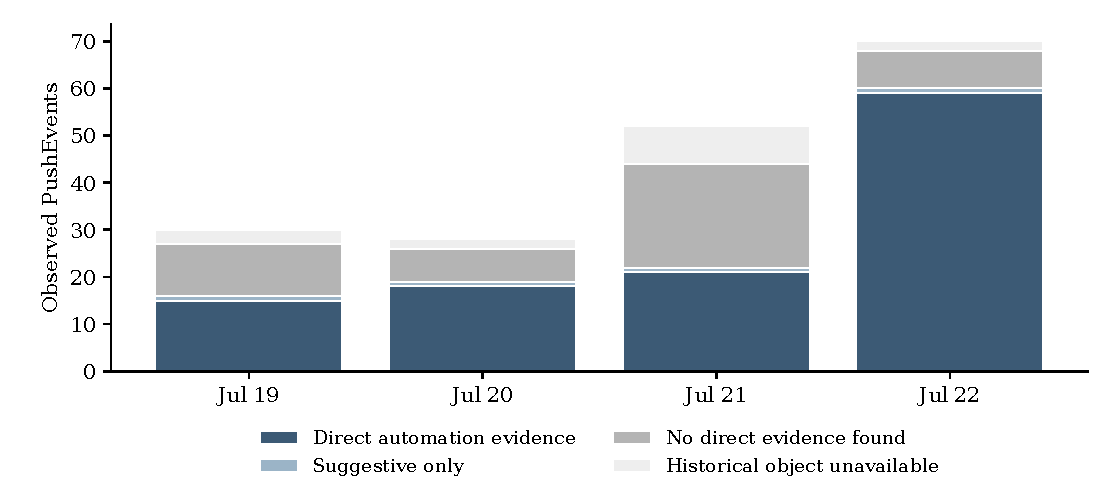
\includegraphics[width=\textwidth]{fig_evidence_automation.pdf}
\fignote{All 180 PushEvents on July 19--22 from the 40 core publishers. Classification concerns the head commit and available historical evidence. Direct evidence requires a machine identity corroborated by messages/files or a matching generating workflow; suggestive patterns and unavailable objects remain separate. No-direct-evidence cases are not certified human activity. Non-push primary events are omitted from this figure but retained in Table~\ref{tab:evidence_audit}.}
\end{figure}

\clearpage
{\footnotesize\setlength{\tabcolsep}{3pt}
\begin{longtable}{@{}p{.065\textwidth}rrp{.13\textwidth}p{.61\textwidth}@{}}
\caption{Individual review of every core-window publisher}\label{tab:evidence_cases}\\
\toprule Case & Events & Auto & Evidence & Basis and qualification \\
\midrule\endfirsthead
\toprule Case & Events & Auto & Evidence & Basis and qualification \\
\midrule\endhead
\bottomrule\endfoot
C002 & 4 & 4 & Direct & GitHub Actions author; generated snake SVG files. \\
C003 & 4 & 4 & Direct & readme-bot; scheduled WakaTime README workflow. \\
C006 & 1 & 0 & Not identified & Kubernetes/project files; no identified automated publishing mechanism. \\
C008 & 3 & 3 & Direct & readme-bot; historical scheduled WakaTime workflow. \\
C014 & 5 & 0 & Not identified & Build-fix commits; CI and stale-issue workflows do not establish automation of these pushes. \\
C021 & 5 & 0 & Not identified & IDE-file removals and a project README; no direct automation evidence. \\
C024 & 8 & 0 & Insufficient & Eight regularly timed profile-repository pushes, but historical objects unavailable; timing alone is insufficient. \\
C039 & 21 & 7 & Direct & Snyk bot heads; dependency-upgrade messages and manifests. \\
C043 & 16 & 16 & Direct & GitHub Actions author; generated snake SVG files. \\
C047 & 3 & 0 & Not identified & Favicon and application changes; no identified automatic publisher. \\
C049 & 10 & 0 & Not identified & Stack/queue exercises and React signup edits; repetitive messages alone do not establish automation. \\
C051 & 3 & 3 & Direct & readme-bot; historical scheduled WakaTime workflow. \\
C062 & 3 & 1 & Direct & Snyk bot head; lucide-react dependency upgrade. \\
C070 & 4 & 4 & Direct & github-actions identity; scheduled video-index pipeline and matching commit message. \\
C083 & 4 & 0 & Suggestive & Four 22:00 UTC host-list updates; an update-and-push script and example crontab exist, but deployment of that schedule is unverified. \\
C084 & 8 & 8 & Direct & github-actions[bot] author; generated deployment output, not inferred from the repository topic. \\
C089 & 4 & 4 & Direct & readme-bot; historical scheduled WakaTime workflow. \\
C093 & 6 & 2 & Direct & Snyk bot heads; mysql2 dependency upgrades. \\
C098 & 1 & 0 & Not identified & Engineering scripts/documents; no identified automatic publisher; commit title uses a local calendar date. \\
C099 & 3 & 0 & Not identified & HTML/CSS fitness-layout edits; no identified automatic publisher. \\
C110 & 2 & 1 & Direct & pyup-bot identity; Sphinx dependency update. \\
C115 & 3 & 1 & Direct & Snyk bot head; dependency-upgrade manifest changes. \\
C116 & 2 & 0 & Not identified & Application project-page edits; no identified automatic publisher. \\
C119 & 2 & 0 & Insufficient & Two CreateEvents only; no commit to inspect. Repository creation is not evidence of coding. \\
C123 & 1 & 0 & Not identified & Java generic-type examples; no identified automatic publisher. \\
C133 & 1 & 0 & Not identified & Three-line HTML change through GitHub UI; GitHub/web-flow is not itself bot evidence. \\
C139 & 7 & 0 & Not identified & Authentication and interface changes; no identified automatic publisher. \\
C140 & 4 & 0 & Mixed & Mixed activity: BibTeX edits and a merge; one onset commit is generated by github-actions[bot] and an exact historical import workflow. \\
C148 & 1 & 0 & Not identified & Power-system code repository; inspected core head resolves a gitignore conflict, not an automatic release. \\
C159 & 1 & 1 & Direct & readme-bot; historical weekly WakaTime workflow. \\
C161 & 7 & 7 & Direct & GitHub Actions author; generated snake SVG files. \\
C177 & 5 & 0 & Insufficient & Historical repository and four core heads unavailable. \\
C183 & 6 & 2 & Direct & Snyk bot heads; Dockerfile vulnerability-fix updates. \\
C222 & 10 & 0 & Not identified & C-sharp interview/data-structure exercises; the term Auto Stack is not evidence of a bot. \\
C226 & 1 & 0 & Not identified & README edits via GitHub UI; no identified automatic publisher. \\
C229 & 1 & 0 & Not identified & React router and page components; no identified automatic publisher. \\
C242 & 4 & 4 & Direct & GitHub Actions author; generated snake SVG files. \\
C260 & 12 & 0 & Not identified & Kotlin multiplatform examples; repeated init messages cover different files and do not establish automation. \\
C272 & 9 & 0 & Insufficient & Three core heads in two repositories unavailable; event combinations alone are insufficient. \\
C273 & 42 & 41 & Direct & All 41 core heads identify pyup-bot and change dependency requirements. \\
\end{longtable}}
\noindent\footnotesize Events counts all primary events on July 19--22; Auto counts only directly evidenced automated push heads. ``Not identified'' is not proof of manual authorship. Mixed denotes the account with a generated onset-authored commit alongside other activity; that generated commit is not itself a core push head. Case IDs map to account/repository/commit URLs and dated API evidence in \texttt{results/evidence\_20261020/individual\_case\_review.csv}. The review is AI-assisted and has not been independently validated by a second reviewer.\normalsize



\clearpage
\subsection{Country-by-country activity and complete domain coverage}

\label{app:country_atlas}

The following figures show every country and every defined repository domain, including cells that do not qualify for a synthetic-control estimate. Cohorts and denominators are fixed before July 18 using the historical-text assignment described in Section~\ref{sec:international_sector_data}. A small or empty cell is shown explicitly; it is not replaced by a zero causal effect. These plots describe measured public activity and do not identify employment industries.

\begin{figure}[H]\centering

\caption{Eligible accounts by country and pre-treatment repository domain}

\label{fig:country_domain_support}

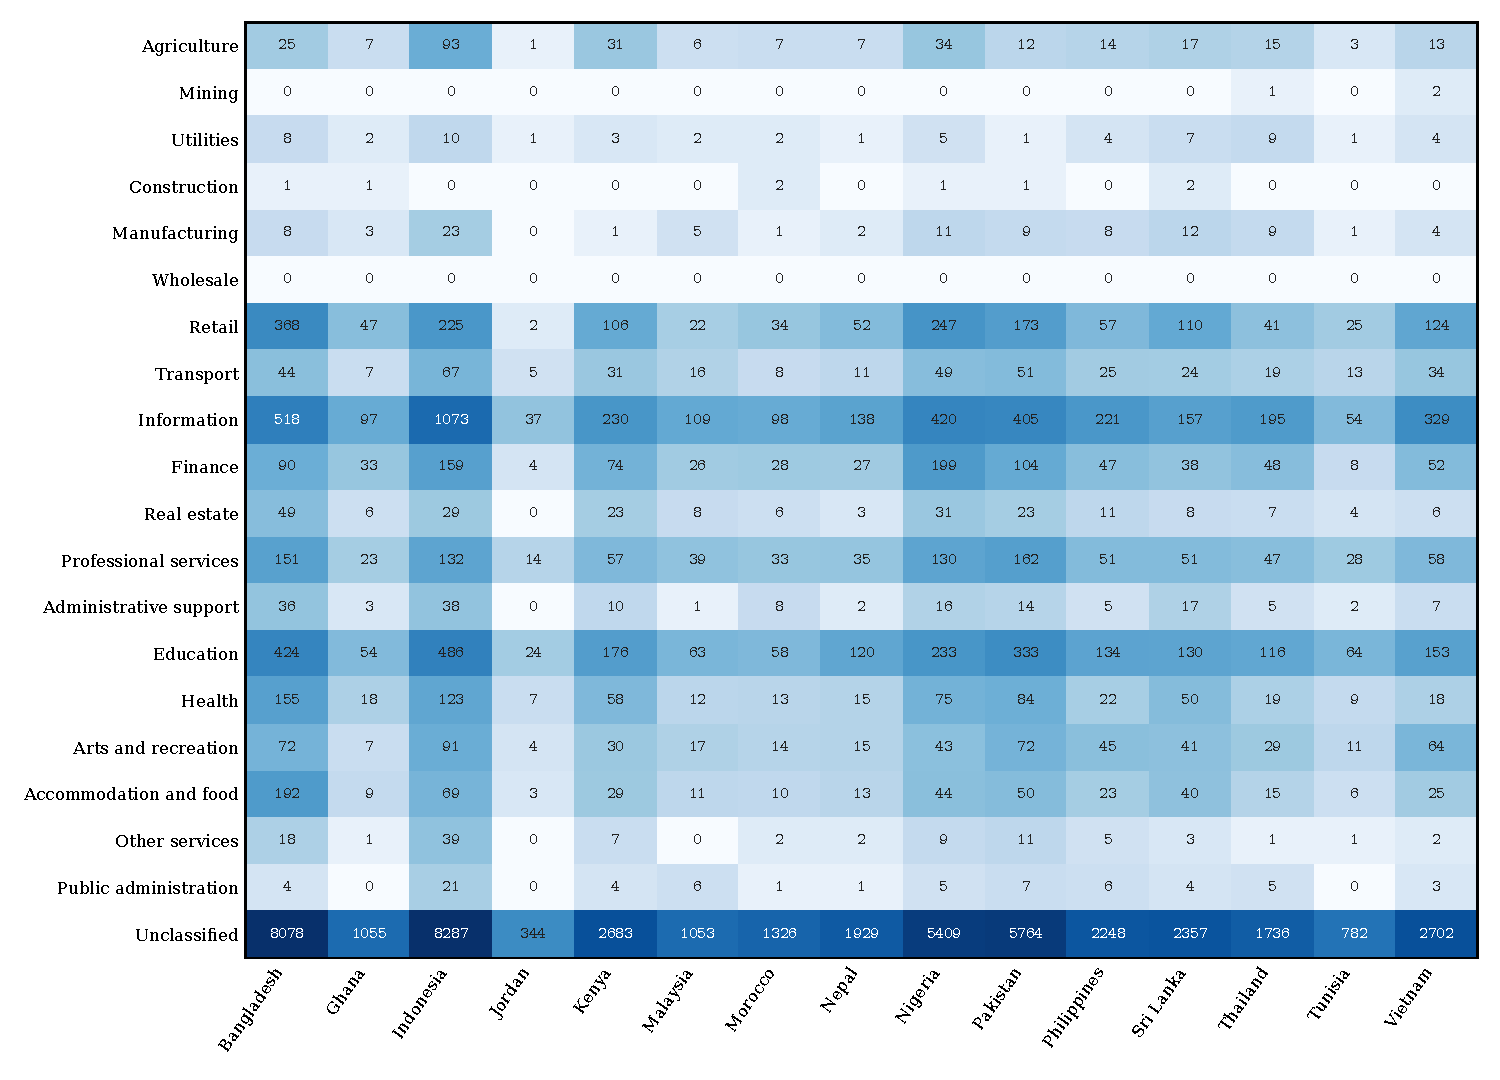
\includegraphics[width=\textwidth]{fig_evidence_country_domain_support.pdf}

\fignote{Numbers are fixed cohort sizes. Colour represents $\log_{10}(1+N)$ for readability. All 59,158 eligible users are assigned exactly once, including the unclassified group. The existing estimation screen requires at least 30 Bangladesh users and five donor countries with at least 30 users each; these descriptive figures apply no such deletion.}

\end{figure}\clearpage

\begin{figure}[p]\centering

\caption{Daily public activity in Bangladesh and every donor country}

\label{fig:country_national}

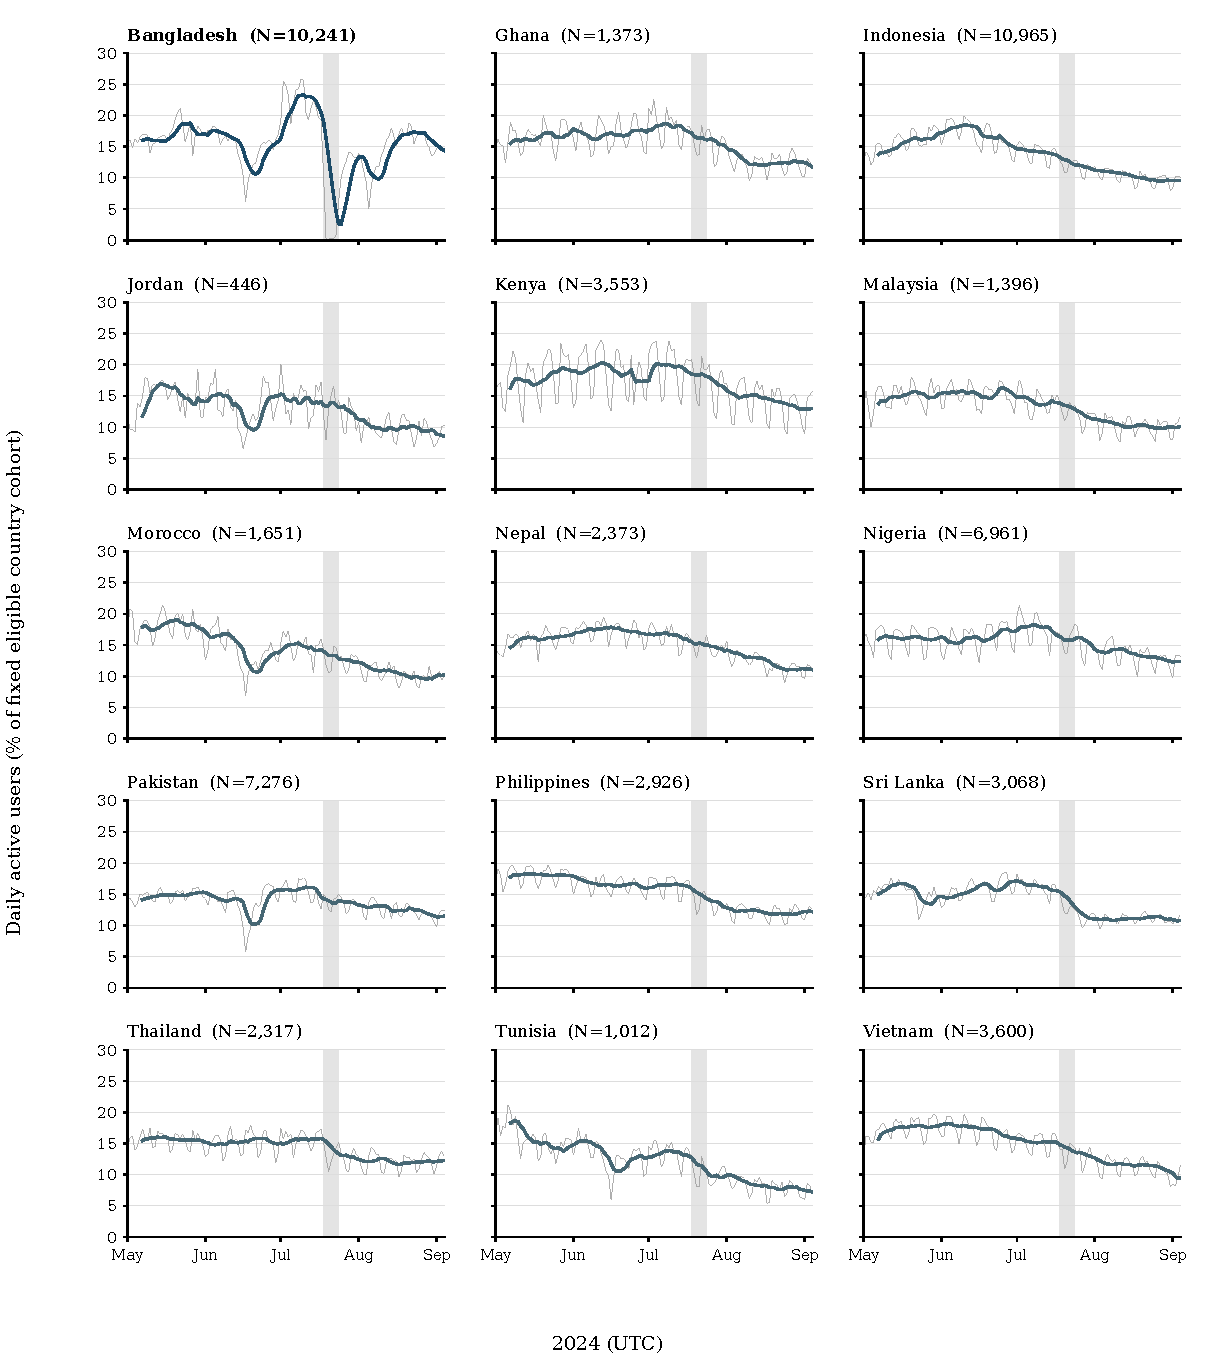
\includegraphics[width=\textwidth,height=.81\textheight,keepaspectratio]{fig_evidence_country_national.pdf}

\fignote{Thin grey lines: daily rates; coloured lines: trailing seven-day means, shown only after seven observations. Grey shading: July 18--23. All days and rates use UTC and the original country denominators. The smoothing is descriptive and is not used to re-estimate the primary model.}

\end{figure}\clearpage

\begin{figure}[p]\centering

\caption{Country-by-country public activity: Agriculture}

\label{fig:atlas_11}

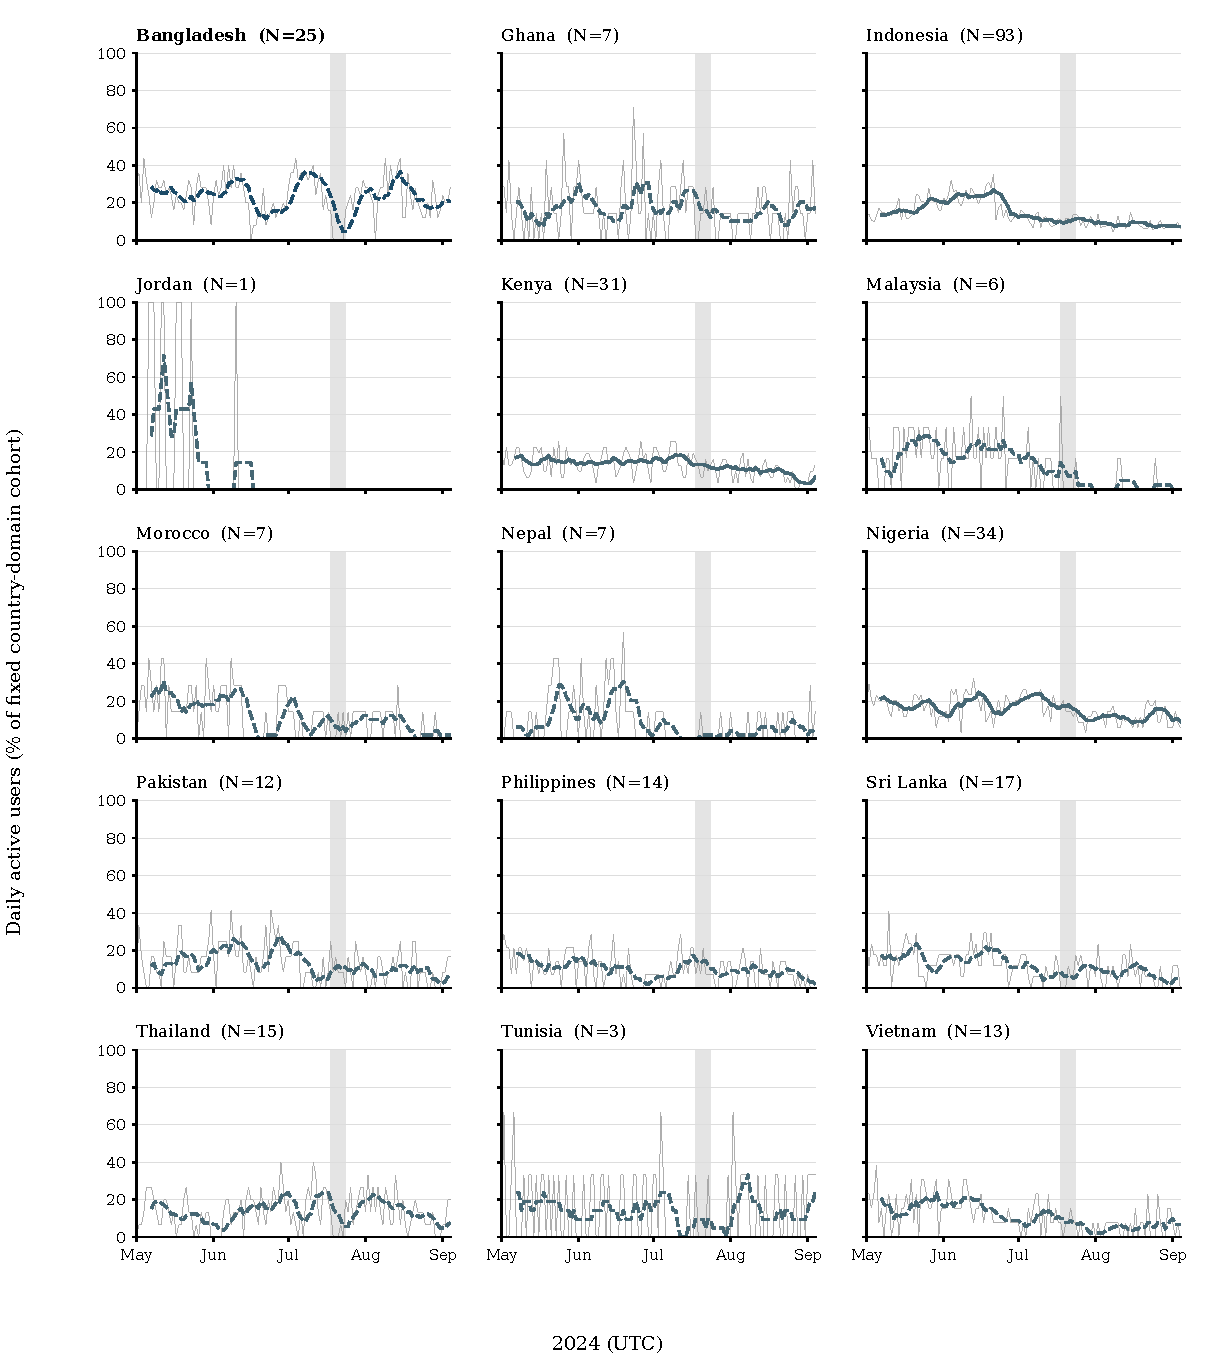
\includegraphics[page=1,width=\textwidth,height=.81\textheight,keepaspectratio]{fig_evidence_country_sectors.pdf}

\fignote{Fixed historical-README cohort, confidence threshold 0.80. Thin grey: daily rates; coloured: trailing seven-day mean. Dashed means indicate fewer than 30 users; empty cells have no assigned users. Scales are common across countries on this page but may differ across domains. Grey shading: July 18--23. The outcome counts each assigned user's primary activity anywhere on GitHub, not only activity in the repository used for assignment.}

\end{figure}\clearpage

\begin{figure}[p]\centering

\caption{Country-by-country public activity: Mining}

\label{fig:atlas_21}

\includegraphics[page=2,width=\textwidth,height=.81\textheight,keepaspectratio]{fig_evidence_country_sectors.pdf}

\fignote{Fixed historical-README cohort, confidence threshold 0.80. Thin grey: daily rates; coloured: trailing seven-day mean. Dashed means indicate fewer than 30 users; empty cells have no assigned users. Scales are common across countries on this page but may differ across domains. Grey shading: July 18--23. The outcome counts each assigned user's primary activity anywhere on GitHub, not only activity in the repository used for assignment.}

\end{figure}\clearpage

\begin{figure}[p]\centering

\caption{Country-by-country public activity: Utilities}

\label{fig:atlas_22}

\includegraphics[page=3,width=\textwidth,height=.81\textheight,keepaspectratio]{fig_evidence_country_sectors.pdf}

\fignote{Fixed historical-README cohort, confidence threshold 0.80. Thin grey: daily rates; coloured: trailing seven-day mean. Dashed means indicate fewer than 30 users; empty cells have no assigned users. Scales are common across countries on this page but may differ across domains. Grey shading: July 18--23. The outcome counts each assigned user's primary activity anywhere on GitHub, not only activity in the repository used for assignment.}

\end{figure}\clearpage

\begin{figure}[p]\centering

\caption{Country-by-country public activity: Construction}

\label{fig:atlas_23}

\includegraphics[page=4,width=\textwidth,height=.81\textheight,keepaspectratio]{fig_evidence_country_sectors.pdf}

\fignote{Fixed historical-README cohort, confidence threshold 0.80. Thin grey: daily rates; coloured: trailing seven-day mean. Dashed means indicate fewer than 30 users; empty cells have no assigned users. Scales are common across countries on this page but may differ across domains. Grey shading: July 18--23. The outcome counts each assigned user's primary activity anywhere on GitHub, not only activity in the repository used for assignment.}

\end{figure}\clearpage

\begin{figure}[p]\centering

\caption{Country-by-country public activity: Manufacturing}

\label{fig:atlas_31-33}

\includegraphics[page=5,width=\textwidth,height=.81\textheight,keepaspectratio]{fig_evidence_country_sectors.pdf}

\fignote{Fixed historical-README cohort, confidence threshold 0.80. Thin grey: daily rates; coloured: trailing seven-day mean. Dashed means indicate fewer than 30 users; empty cells have no assigned users. Scales are common across countries on this page but may differ across domains. Grey shading: July 18--23. The outcome counts each assigned user's primary activity anywhere on GitHub, not only activity in the repository used for assignment.}

\end{figure}\clearpage

\begin{figure}[p]\centering

\caption{Country-by-country public activity: Wholesale}

\label{fig:atlas_42}

\includegraphics[page=6,width=\textwidth,height=.81\textheight,keepaspectratio]{fig_evidence_country_sectors.pdf}

\fignote{Fixed historical-README cohort, confidence threshold 0.80. Thin grey: daily rates; coloured: trailing seven-day mean. Dashed means indicate fewer than 30 users; empty cells have no assigned users. Scales are common across countries on this page but may differ across domains. Grey shading: July 18--23. The outcome counts each assigned user's primary activity anywhere on GitHub, not only activity in the repository used for assignment.}

\end{figure}\clearpage

\begin{figure}[p]\centering

\caption{Country-by-country public activity: Retail}

\label{fig:atlas_44-45}

\includegraphics[page=7,width=\textwidth,height=.81\textheight,keepaspectratio]{fig_evidence_country_sectors.pdf}

\fignote{Fixed historical-README cohort, confidence threshold 0.80. Thin grey: daily rates; coloured: trailing seven-day mean. Dashed means indicate fewer than 30 users; empty cells have no assigned users. Scales are common across countries on this page but may differ across domains. Grey shading: July 18--23. The outcome counts each assigned user's primary activity anywhere on GitHub, not only activity in the repository used for assignment.}

\end{figure}\clearpage

\begin{figure}[p]\centering

\caption{Country-by-country public activity: Transport}

\label{fig:atlas_48-49}

\includegraphics[page=8,width=\textwidth,height=.81\textheight,keepaspectratio]{fig_evidence_country_sectors.pdf}

\fignote{Fixed historical-README cohort, confidence threshold 0.80. Thin grey: daily rates; coloured: trailing seven-day mean. Dashed means indicate fewer than 30 users; empty cells have no assigned users. Scales are common across countries on this page but may differ across domains. Grey shading: July 18--23. The outcome counts each assigned user's primary activity anywhere on GitHub, not only activity in the repository used for assignment.}

\end{figure}\clearpage

\begin{figure}[p]\centering

\caption{Country-by-country public activity: Information}

\label{fig:atlas_51}

\includegraphics[page=9,width=\textwidth,height=.81\textheight,keepaspectratio]{fig_evidence_country_sectors.pdf}

\fignote{Fixed historical-README cohort, confidence threshold 0.80. Thin grey: daily rates; coloured: trailing seven-day mean. Dashed means indicate fewer than 30 users; empty cells have no assigned users. Scales are common across countries on this page but may differ across domains. Grey shading: July 18--23. The outcome counts each assigned user's primary activity anywhere on GitHub, not only activity in the repository used for assignment.}

\end{figure}\clearpage

\begin{figure}[p]\centering

\caption{Country-by-country public activity: Finance}

\label{fig:atlas_52}

\includegraphics[page=10,width=\textwidth,height=.81\textheight,keepaspectratio]{fig_evidence_country_sectors.pdf}

\fignote{Fixed historical-README cohort, confidence threshold 0.80. Thin grey: daily rates; coloured: trailing seven-day mean. Dashed means indicate fewer than 30 users; empty cells have no assigned users. Scales are common across countries on this page but may differ across domains. Grey shading: July 18--23. The outcome counts each assigned user's primary activity anywhere on GitHub, not only activity in the repository used for assignment.}

\end{figure}\clearpage

\begin{figure}[p]\centering

\caption{Country-by-country public activity: Real estate}

\label{fig:atlas_53}

\includegraphics[page=11,width=\textwidth,height=.81\textheight,keepaspectratio]{fig_evidence_country_sectors.pdf}

\fignote{Fixed historical-README cohort, confidence threshold 0.80. Thin grey: daily rates; coloured: trailing seven-day mean. Dashed means indicate fewer than 30 users; empty cells have no assigned users. Scales are common across countries on this page but may differ across domains. Grey shading: July 18--23. The outcome counts each assigned user's primary activity anywhere on GitHub, not only activity in the repository used for assignment.}

\end{figure}\clearpage

\begin{figure}[p]\centering

\caption{Country-by-country public activity: Professional services}

\label{fig:atlas_54}

\includegraphics[page=12,width=\textwidth,height=.81\textheight,keepaspectratio]{fig_evidence_country_sectors.pdf}

\fignote{Fixed historical-README cohort, confidence threshold 0.80. Thin grey: daily rates; coloured: trailing seven-day mean. Dashed means indicate fewer than 30 users; empty cells have no assigned users. Scales are common across countries on this page but may differ across domains. Grey shading: July 18--23. The outcome counts each assigned user's primary activity anywhere on GitHub, not only activity in the repository used for assignment.}

\end{figure}\clearpage

\begin{figure}[p]\centering

\caption{Country-by-country public activity: Administrative support}

\label{fig:atlas_56}

\includegraphics[page=13,width=\textwidth,height=.81\textheight,keepaspectratio]{fig_evidence_country_sectors.pdf}

\fignote{Fixed historical-README cohort, confidence threshold 0.80. Thin grey: daily rates; coloured: trailing seven-day mean. Dashed means indicate fewer than 30 users; empty cells have no assigned users. Scales are common across countries on this page but may differ across domains. Grey shading: July 18--23. The outcome counts each assigned user's primary activity anywhere on GitHub, not only activity in the repository used for assignment.}

\end{figure}\clearpage

\begin{figure}[p]\centering

\caption{Country-by-country public activity: Education}

\label{fig:atlas_61}

\includegraphics[page=14,width=\textwidth,height=.81\textheight,keepaspectratio]{fig_evidence_country_sectors.pdf}

\fignote{Fixed historical-README cohort, confidence threshold 0.80. Thin grey: daily rates; coloured: trailing seven-day mean. Dashed means indicate fewer than 30 users; empty cells have no assigned users. Scales are common across countries on this page but may differ across domains. Grey shading: July 18--23. The outcome counts each assigned user's primary activity anywhere on GitHub, not only activity in the repository used for assignment.}

\end{figure}\clearpage

\begin{figure}[p]\centering

\caption{Country-by-country public activity: Health}

\label{fig:atlas_62}

\includegraphics[page=15,width=\textwidth,height=.81\textheight,keepaspectratio]{fig_evidence_country_sectors.pdf}

\fignote{Fixed historical-README cohort, confidence threshold 0.80. Thin grey: daily rates; coloured: trailing seven-day mean. Dashed means indicate fewer than 30 users; empty cells have no assigned users. Scales are common across countries on this page but may differ across domains. Grey shading: July 18--23. The outcome counts each assigned user's primary activity anywhere on GitHub, not only activity in the repository used for assignment.}

\end{figure}\clearpage

\begin{figure}[p]\centering

\caption{Country-by-country public activity: Arts and recreation}

\label{fig:atlas_71}

\includegraphics[page=16,width=\textwidth,height=.81\textheight,keepaspectratio]{fig_evidence_country_sectors.pdf}

\fignote{Fixed historical-README cohort, confidence threshold 0.80. Thin grey: daily rates; coloured: trailing seven-day mean. Dashed means indicate fewer than 30 users; empty cells have no assigned users. Scales are common across countries on this page but may differ across domains. Grey shading: July 18--23. The outcome counts each assigned user's primary activity anywhere on GitHub, not only activity in the repository used for assignment.}

\end{figure}\clearpage

\begin{figure}[p]\centering

\caption{Country-by-country public activity: Accommodation and food}

\label{fig:atlas_72}

\includegraphics[page=17,width=\textwidth,height=.81\textheight,keepaspectratio]{fig_evidence_country_sectors.pdf}

\fignote{Fixed historical-README cohort, confidence threshold 0.80. Thin grey: daily rates; coloured: trailing seven-day mean. Dashed means indicate fewer than 30 users; empty cells have no assigned users. Scales are common across countries on this page but may differ across domains. Grey shading: July 18--23. The outcome counts each assigned user's primary activity anywhere on GitHub, not only activity in the repository used for assignment.}

\end{figure}\clearpage

\begin{figure}[p]\centering

\caption{Country-by-country public activity: Other services}

\label{fig:atlas_81}

\includegraphics[page=18,width=\textwidth,height=.81\textheight,keepaspectratio]{fig_evidence_country_sectors.pdf}

\fignote{Fixed historical-README cohort, confidence threshold 0.80. Thin grey: daily rates; coloured: trailing seven-day mean. Dashed means indicate fewer than 30 users; empty cells have no assigned users. Scales are common across countries on this page but may differ across domains. Grey shading: July 18--23. The outcome counts each assigned user's primary activity anywhere on GitHub, not only activity in the repository used for assignment.}

\end{figure}\clearpage

\begin{figure}[p]\centering

\caption{Country-by-country public activity: Public administration}

\label{fig:atlas_92}

\includegraphics[page=19,width=\textwidth,height=.81\textheight,keepaspectratio]{fig_evidence_country_sectors.pdf}

\fignote{Fixed historical-README cohort, confidence threshold 0.80. Thin grey: daily rates; coloured: trailing seven-day mean. Dashed means indicate fewer than 30 users; empty cells have no assigned users. Scales are common across countries on this page but may differ across domains. Grey shading: July 18--23. The outcome counts each assigned user's primary activity anywhere on GitHub, not only activity in the repository used for assignment.}

\end{figure}\clearpage

\begin{figure}[p]\centering

\caption{Country-by-country public activity: Unclassified}

\label{fig:atlas_Unclassified}

\includegraphics[page=20,width=\textwidth,height=.81\textheight,keepaspectratio]{fig_evidence_country_sectors.pdf}

\fignote{Fixed historical-README cohort, confidence threshold 0.80. Thin grey: daily rates; coloured: trailing seven-day mean. Dashed means indicate fewer than 30 users; empty cells have no assigned users. Scales are common across countries on this page but may differ across domains. Grey shading: July 18--23. The outcome counts each assigned user's primary activity anywhere on GitHub, not only activity in the repository used for assignment.}

\end{figure}\clearpage

